\documentclass[11pt,a4paper,dvipsnames,twosided]{article}
\usepackage[deliverable]{IOHKCoverPage}

% data for Deliverable header -- added by KH from an EU H2020 project template
\DeliverableNumber{SL-D1}
\DeliverableTitle{Design Specification for Delegation and Incentives in Cardano}{Delegation/Incentives Design Spec.}
\DeliverableResponsible{Formal Methods Team}
\EditorName{Philipp Kant, \IOHK}
\Authors{Philipp Kant   \quad \texttt{<philipp.kant@iohk.io>}
   \\[1em]
   Lars Br\"unjes \quad \texttt{<lars.bruenjes@iohk.io>}
   \\[1em]
   Duncan Coutts  \quad \texttt{<duncan.coutts@iohk.io>}
}
\DueDate{28$^{\textrm{st}}$ February 2020}
\SubmissionDate{28$^{\textrm{th}}$ February 2020}{2020/02/28}
\LeaderName{Philipp Kant, \IOHK}
\InstitutionAddress{\IOHK}
\Version{1.10}
\Project{Shelley Ledger}
\DisseminationPU

\usepackage[margin=2.5cm]{geometry}
\usepackage{lscape}
%\usepackage[a-1b]{pdfx}
\usepackage{microtype}
\usepackage{mathpazo} % nice fonts
\usepackage{amsmath, amssymb, stmaryrd, latexsym, mathtools}
\usepackage{extarrows}
\usepackage{slashed}
% \usepackage[colon]{natbib}
\newcommand{\citep}[1]{\cite{#1}}
\usepackage{todonotes}
\usepackage[unicode=true,pdftex,pdfa,colorlinks=true]{hyperref}
\usepackage[capitalise,noabbrev,nameinlink]{cleveref}
\usepackage{titlesec}
\hypersetup{
  pdftitle={Design Specification for Delegation and Incentives in Cardano},
  pdfauthor={Philipp Kant, Lars Brünjes, Duncan Coutts},
  breaklinks=true,
  bookmarks=true,
  colorlinks=false,
  linkcolor={blue},
  citecolor={blue},
  urlcolor={blue},
  linkbordercolor={white},
  citebordercolor={white},
  urlbordercolor={white}
}
\usepackage{float}
\floatstyle{boxed}
\restylefloat{figure}
% For making figures
\usepackage{tikz}
\usetikzlibrary{positioning}
\usetikzlibrary{arrows.meta}
\usetikzlibrary{calc}

\setcounter{secnumdepth}{4}
\titleformat{\paragraph}
            {\normalfont\normalsize\bfseries}{\theparagraph}{1em}{}
            \titlespacing*{\paragraph}
                          {0pt}{3.25ex plus 1ex minus .2ex}{1.5ex plus .2ex}

\DeclareMathOperator{\dom}{dom}
\DeclareMathOperator{\range}{range}

\newcommand*\ema[2]{\left\langle {#1} \right\rangle_{{#2}}}
\newcommand*\mean[1]{\overline{#1}}

\newcommand\pbar{\overline{p}}
\newcommand\Nbar{\overline{N}}

\begin{document}


  \cleardoublepage%
  \tableofcontents%
  \listoffigures%
  \clearpage%

  \begin{changelog}
\change{2018-12-18}{PK, LB, DC}{FM (IOHK)}{First version that is considered stable enough to warrant V1. Some things still
need to be pinned down.}
\change{2019-01-07}{PK, LB, DC}{FM (IOHK)}{
Changes after the first day of the Berlin workshop. TTL for transactions; stakepool registration.
% - Add todo to clarify stakepool metadata
% - Add section on TTL for transactions
% - Elaboration and slight change to stake pool registration.

%   After the first day of discussions in Berlin, we came to the conclusions that

%   - we need a \emph{registered} staking key to collect rewards
%   - this should \emph{not} be the same key that's used for participating in the
%     protocol. For participation in the protocol, we want cold and operational
%     keys, and using the same key to withdraw rewards is detrimental.
%   - We needed more elaboration on the multiple owner use case, emphasising that
%     the rewards for all owners are given to the operator.
% - Resolved several todo items
% - Include git revision in documents
% - Explain why pool registration will not be censored.
}
\change{2019-01-08}{PK, LB, DC}{FM (IOHK)}{Changes after the second day of the Berlin workshop.
Avoid Contention at Epoch Boundary. Refunds after stake pool retirement. Clarifications and corrections.}
% - Avoid overloading the term "pool"
% - Clarify that Treasury is a Sink for now.
% - Avoid Contention at Epoch Boundary
% - Decision made: refund for stake pool paid after retirement.
% - Update to non-refundable part of deposits

%   We figured out in the formal spec how to incrementally add the non-refundable
%   part to the reward pool of all the relevant epochs, which is fairer than
%   adding all of it to the reward pool where the resource is released.
% - Correction: we're introducing four address types, not three
%}
\change{2019-03-01}{PK, LB, DC}{FM (IOHK)}{Incorporating further input from the workshop in Berlin, and following discussions,
into the document. Transactions have to have at least one UTxO style input; stake pool metadata formats; choice of KES scheme; deposits information; clarify certificate replay protection; fix rewards to treasury for unregistered stake pool key; update  block validity to require operational key;
additions to Operational Key section.}

% - Decision: transactions have to have at least one UTxO style input

% - Update: Stake pool metadata

%   Specify the format for the metadata, and how it is provided. Streamlined the
%   different sections that touch stake pool metadata.
% - Elaborating further on why stake pool registrations will not be censored.
% - Capture choice of KES scheme in design doc.
% - Streamlining information on deposits

%     Replacing an explanation of the concept with a link to the section where it's
%     already explained.
% - Elaborate on certificate replay protection

%     The paragraph was not entirely true, it said there was only one possible source
%     of funds in addition to UTxO entries, but with rewards accounts, there is
%     another one.
% - Fix that rewards go to treasury if reward key unregistered.

%     We can not move them to the rewards pool -- if we did, it would create an
%     incentive for all other leaders to censor a certificate that caused the pool to
%     use a valid certificate.
% - Update block validity to require operational key
% - Additions to Operational Key section
%     - They are compulsory
%     - They will use KES
%     - Operational Key Certificates will expire, to encourage key rotation
%     - Slight Change in validity rules
% - Add FAQ section to the delegation design doc
% - Add a couple of todo entries
% }
\change{2019-04-05}{PK, LB, DC}{FM (IOHK)}{Rewrote the chapter on rewards.
%
% We had lots of discussions about how to properly account for the performance of
% pools, particularly in Praos where the actual performance is not observable due
% to the private leader schedule. We finally converged to a solution, leading to a
% re-write of the incentives section.

% Also, changed the title of the document, and made the capitalisation of ada
% consistent.
}
\change{2019-04-08}{PK, LB, DC}{FM (IOHK)}{General review of the document.
Mostly small things. Consistent wording, spelling, readability, removed some
obsolete things.
%
% Removed the remaining todo items. Decisions we still need to make are now
% tracked on github instead.
%
% Moved the section on detecting stale stake into an appendix, and changed it to
% reflect the design where stake that is not delegated to an active pool is
% ignored (which solves the problem of stale stake to a large degree).
}
\change{2019-04-11}{PK, LB, DC}{FM (IOHK)}{Some subtle corrections in the rewards chapter after review by Aikaterina.
First version officially published on the IOHK blog.}
\change{2019-05-17}{PK, LB, DC}{FM (IOHK)}{Some clarifications in response to review by the auditors.}
\change{2019-06-07}{PK, LB, DC}{FM (IOHK)}{Update section on script addresses.}
\change{2019/10/09}{Kevin Hammond}{FM (IOHK)}{Added standard cover page.}
\change{2020-02-28}{PK}{FM (IOHK)}{Clarify when to use active/total stake.}
\change{2020/03/11}{DC}{FM (IOHK)}{Document the metadata feature.}
\change{2020-06-12}{PK}{FM (IOHK)}{Rewrite chapter on addresses. Now includes
  multi-sig, and is clearer about the distinction of payment addresses, stake
  addresses, credentials.}
\end{changelog}

\clearpage%
\begin{landscape}
\floatstyle{plain}
\restylefloat{figure}
\begin{figure*}
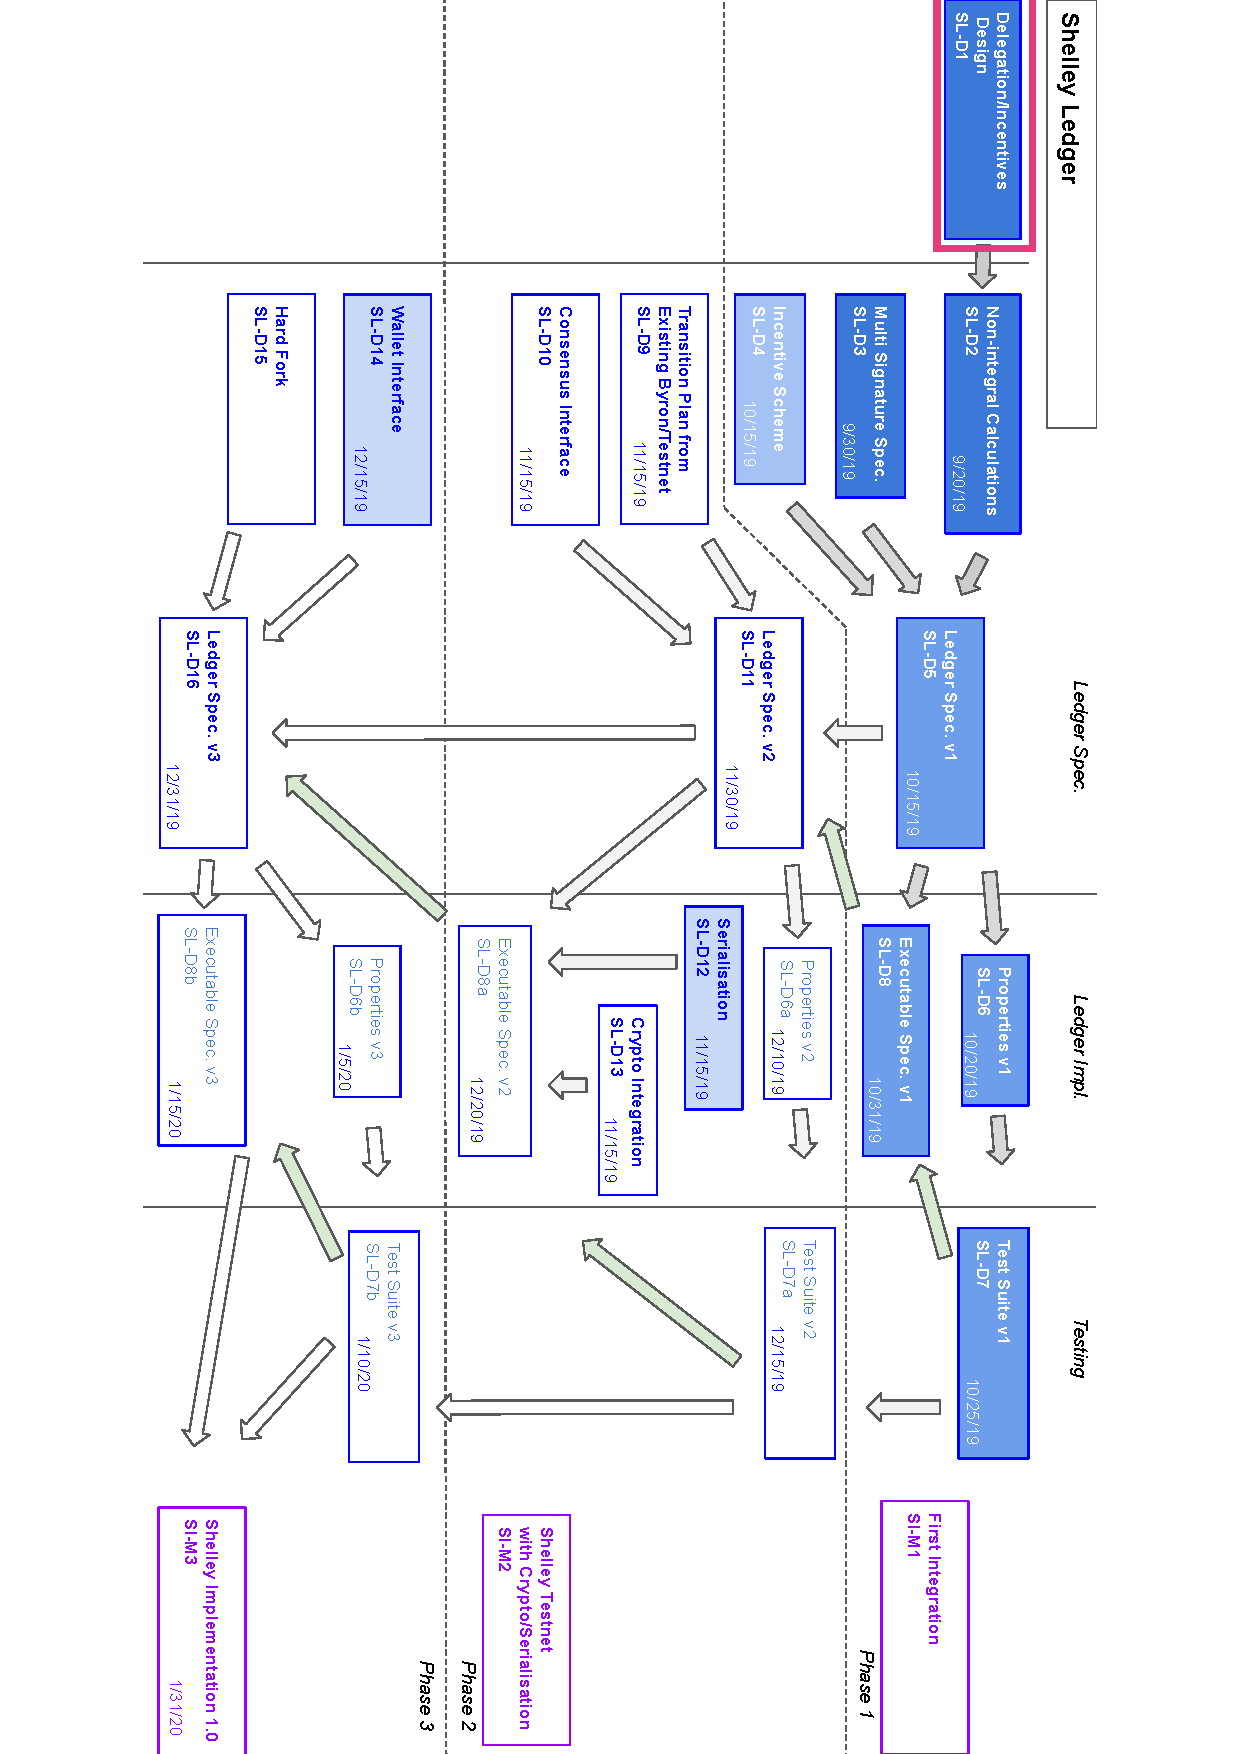
\includegraphics[scale=0.8,angle=90]{d1-depends.pdf}
\caption{Positioning of this Deliverable (outlined in red).}
\end{figure*}
\end{landscape}
\floatstyle{boxed}
\restylefloat{figure}
\cleardoublepage
% \begin{center}
%   \large{Executive Summary}
% \end{center}

% \noindent
% This document provides a formal specification of the Cardano ledger for use in the Shelley implementation.
% It is intended to form the basis for an executable specification that will be the basis of the initial
% release.
% \cleardoublepage
\renewcommand{\thepage}{\arabic{page}}
\setcounter{page}{1}

\title{Engineering Design Specification \\
  for Delegation and Incentives \\
  in Cardano--Shelley \\
  {\large \sc An IOHK technical report}}

\author{Philipp Kant   \\ {\small \texttt{philipp.kant@iohk.io}} \\
   \and Lars Br\"unjes \\ {\small \texttt{lars.bruenjes@iohk.io}} \\
   \and Duncan Coutts  \\ {\small \texttt{duncan@well-typed.com}} \\
                          {\small \texttt{duncan.coutts@iohk.io}}}
\maketitle

\begin{abstract}
This document describes the requirements and design for a delegation and
incentives mechanism to be used in the Shelley release of Cardano.
\end{abstract}

\section*{List of Contributors}
\label{acknowledgements}

Lars Br\"unjes, Jared Corduan, Duncan Coutts, Matthias G\"udemann,
Philipp Kant, Dimitris Karakostas, Aggelos Kiayias, Elias Koutsoupias,
Mario Larangeira, Damian Nadales, Aikaterini-Panagiota Stouka.

%\tableofcontents
%\listoffigures
%% Not in final version -- KH
%\listoftodos

\section{Purpose}
\label{purpose}

Delegation will allow holders of ada to transfer their rights to participate in
the proof of stake (\emph{PoS}) protocol to \emph{stake pools}. Stake pools are
run by \emph{stake pool operators} (sometimes also called \emph{pool leaders},
though we try to avoid the term in this document to avoid confusion with slot
leaders), and a person delegating to a stake pool is called \emph{delegator},
\emph{member}, or \emph{participant} of a stake pool.

Introducing delegation is important to increase the stability and
performance of the system:

\begin{itemize}
\item
  We cannot expect every holder of ada to continuously run a node that
  is well-connected to the rest of the network, in order to write a
  block on rare occasions. Some users might lack the expertise to do so.
  Most users will not have enough stake to warrant running their own
  node. Delegation allows all holders of ada to participate in the
  protocol, regardless of their technical abilities and the amount of
  stake that they hold. Thus, we expect less stake to be offline, making
  the system faster and more resilient against an adversary.
\item
  Even if every user were to run a node that was online all the time, it
  would be hard to keep all those nodes well enough in sync to avoid
  forks and still keep a short slot length. Our delegation design is
  aimed at keeping the number of nodes that produce a significant amount
  of blocks reasonably small (about 100 or 1000 nodes), so that effective
  communication between them is feasible.
\end{itemize}

This document covers the design of necessary additions to Cardano in
order to support and incentivise delegation.

\section{Requirements}
\label{requirements}

The delegation mechanism should meet a number of requirements. They can
be grouped into:

\begin{itemize}
\item
  functional requirements that the delegation system should provide;
\item
  requirements to the security (both of the overall system and the funds
  of individual users);
\item
  non-functional requirements; and
\item
  existing features that should not be impeded when we add delegation to
  the system.
\end{itemize}

Requirements specific to the rewards distribution mechanism are
discussed separately in \cref{rewards}.

\subsection{Functional Requirements}
\label{functional-requirements}

\subsubsection{Proof of Eligibility}
\label{proof-of-eligibility}

Any slot leader -- and in particular stake pool operators, who are
elected through stake that is delegated to them -- should be able to
prove when they are eligible to produce a block in a given slot.

\subsubsection{Visibility of Delegation on the Blockchain}
\label{visibility-of-delegation-on-the-blockchain}

We enable stake pools to automatically share their rewards with the
delegators. In order to do this, there must be evidence for the
delegation happening. Furthermore, we want the sharing of rewards to be
enforced by the protocol, so the evidence must be recorded on the
blockchain.

\subsubsection{Restricting Chain Delegation}
\label{restricting-chain-delegation}

We do not want to allow stake to be re-delegated along a chain
arbitrarily. We can admit some level of indirection, but not more than
necessary to meet the rest of the requirements.

One reason that we do not want arbitrary chain delegation is that it
makes it harder for delegators to figure out who is ultimately
controlling their stake. Another is that unlimited chain delegation
could open up a Denial-of-Service (DoS) attack vector on the system,
where the attacker posts long delegation chains in order to slow down
processes that depend on delegation, such as leader election or rewards
sharing.

We must also have a mechanism to prevent cycles (such as A delegates to
B, and B delegates to A) which would introduce ambiguity to the question
of who manages stake in the end.

\subsubsection{Cheap Re-Delegation}
\label{cheap-re-delegation}

Changing delegation preferences should be as cheap as possible (while
still using appropriate fees to prevent a denial of service attack on
the blockchain).

\subsubsection{Neutral Addresses}
\label{neutral-addresses}

We should provide addresses that can hold value, but do not contribute
to the PoS protocol. Those might be appropriate for use by exchanges,
which will hold large amounts of value, without legally owning it.

\subsubsection{Multi-Signature Addresses}
\label{multi-sig-addresses}

We should provide addresses that can hold value that are owned by
multiple people, such that the signatures from some subset are required
to spend from those addresses. This needs to enable addresses where
signatures are required from any N of a pre-determined set of M keys.

\subsubsection{Multi-Signature Delegation}
\label{multi-sig-delegation}

We should provide the ability to declare that delegating the stake
rights for certain funds should require multiple signatures.

This should be as expressive as the multi-signature support for
addresses. It should be an independent choice: a multi-signature
address can use a single signature for its stake rights, or a
different choice of multi-signature threshold N and key set M.

\subsection{Security Requirements}
\label{security-requirements}

\subsubsection{Sybil Attack Protection at Stake Pool Level}
\label{sybil-attack-protection-at-stake-pool-level}

It is conceivable that an adversary might try to take over the
network by registering a large number of stake pools, hoping to
accumulate enough stake to mount an attack just by people randomly
delegating to them.

This Sybil attack on the level of stake pools should be made infeasible,
by requiring stake pool operators to allocate a finite resource to each
individual pool they register. In particular, this resource cannot be
the cost of operating a node, since it is possible to run multiple pools
with one node, so that cost would be constant in the number of pools an
adversary is registering.

\subsubsection{Address Non-malleability}
\label{address-nonmalleability}

The system should provide protection against the following attack:

\begin{description}
\item[Changing Delegation through Address Malleability]
Suppose that Alice makes a payment to Bob. In preparation, Bob transmits
an address belonging to his wallet to Alice, and expects Alice to pay to
that address. If his wallets later on shows that his balance is
increased by the expected amount, he considers that transaction to be
successful. An attacker that wants to increase their influence on the
PoS protocol changes the address that Bob sends in such a way that funds
in that address are delegated to the attacker, but the funds still show
up in Bob's wallet.

The attack is considered successful if the staking rights for the
transferred money belong to the attacker after the transaction, without
Alice and Bob noticing the attack.
\end{description}

\subsubsection{Public Spending Keys Should not be Disclosed Prematurely}
\label{public-spending-keys-should-not-be-disclosed-prematurely}

Delegation of stake should not involve revealing the public spending key (other
than the public key hash, which is already visible from the address itself). The
public spending key should only be revealed once the funds that are controlled
by the corresponding private key are actually transferred to another address.

\subsubsection{Mitigate Key Exposure}
\label{mitigate-key-exposure}

A node run by a stake pool will need to have some key that controls all
the delegated stake, in order to sign blocks. In case of an incident
where the node is compromised, it should be possible for the stake pool
operator to revoke the key, and replace it with a new one. This should
not require any action by the delegators.

\subsubsection{Handle Inactive Stake Pools}
\label{handle-inactive-stake-pools}

We anticipate that a stake pool operator can cease to operate -- whether
they lost their keys, lost interest, etc. We want to minimise the
effect of this to the security and liveness of the system.


Note that this does not only concern large stakeholders. The cumulative effect
of a large number of small stakeholders having their stake be inactive also has
to be considered.


\subsubsection{Avoid Hard Transition}
\label{avoid-hard-transition}

When we make the switch from Byron (where all stake is delegated to the
nodes controlled by the Cardano Foundation, Emurgo, and IOHK) to Shelley
(where ada holders have the freedom to control their stake), we should
avoid a scenario where a significant amount of stake is suddenly
offline.

This could happen if we automatically revoked the automatic delegation
to the core nodes of the Byron network.

\subsubsection{Change Delegation Without Spending Key}
\label{change-delegation-without-spending-key}

Users of a cold wallet, such as a paper wallet or a hardware wallet,
should be able to delegate the stake corresponding to the funds in the
cold wallet without using its spending key.

\subsection{Non-functional Requirements}
\label{non-functional-requirements}

\subsubsection{Asymptotic space and time complexity}
\label{asymptotic-space-and-time-complexity}

All the changes to delegation are changes in the rules that define what
it means to be a valid Cardano blockchain. These rules must be
computable, and must be computable with reasonable space and time
complexity.

\subsubsection{Minimise economic attacks}
\label{minimise-economic-attacks}

An economic attack on a system arises where the costs incurred by the
operators of a system are not covered by fees on the users of the
system. Such situations allow users to impose costs on operators without
paying that full cost themselves. In severe cases this can lead to
operators dropping out and the system collapsing.

Cardano currently has transaction fees which are intended to cover the
processing and long term storage cost of transactions. There are no fees
however for the memory cost of tracking the current accumulated chain
state, in particular the UTxO. In addition, the new mechanisms
introduced for delegation add additional state that must be tracked.
Moving from federated operation to fully decentralised operation may
increase the incentive to exploit economic attacks, so it is important
to address the existing unaccounted operator costs as well as new costs.

\subsection{Requirements to Preserve Existing Features}
\label{requirements-to-preserve-existing-features}

\subsubsection{Master Recovery Key}
\label{master-recovery-key}

The whole wallet should be recoverable from one single key (without any
additional information, such as the delegation preferences of the
wallet).

The computational complexity of the recovery process should not be worse
than logarithmic in the number of addresses appearing on the blockchain,
and linear in the number of addresses in the wallet.

\subsubsection{Address Recognition}
\label{address-recognition}

An HD wallet should be able to recognise its addresses in the UTxO, so
that it can report balances and transaction histories to the user.

\subsubsection{Wallet should be Runnable on Independent Devices}
\label{wallet-should-be-runnable-on-independent-devices}

Different user interfaces, running on different devices, should be able
to access and control the same wallet, without transferring state
between them.

We will accept some degradation of behaviour when running the wallet on
different devices:

\begin{itemize}
\item
  Both copies might generate the same fresh addresses
\item
  There can be differences in the reported balance while there are
  transactions in flight that only one of the two copies has knowledge
  of. In particular, when one copy sends a transaction, that transaction
  will only affect the balance reported by the other wallet once it is
  recorded on the blockchain.
\item
  If the wallets use different delegation preferences, funds sent to the
  wallet might end up being delegated to different pools.
\end{itemize}

\subsubsection{Maintain Privacy}
\label{maintain-privacy}

HD Wallets maintain some level of privacy by using multiple addresses
that are not obviously and publicly tied to the same wallet. Delegating
stake should not necessarily link the addresses in the wallet of a
delegator.

\subsubsection{Short Addresses}
\label{short-addresses}

Adding delegation to the system should not increase the length of
addresses more than necessary. Ideally, we should use the opportunity of having
to modify the address scheme to come up with an address length that is
even shorter than in Byron.

\subsubsection{No lookup of old blocks}
\label{no-lookup-of-old-blocks}

The current Cardano design allows, in principle, an implementation of a
node that discards blocks after a period of time so that it only needs
to keep a limited number of recent blocks. This is true in part because
nothing in the existing validation rules requires looking up arbitrary
old blocks. All information necessary for validation can be accumulated
in a running state, in a \texttt{foldl} style. This is a useful design
property to retain.

\subsection{Design Goals}
\label{design-goals}

\subsubsection{No Special Wallet for Stake Pool Operators}
\label{no-special-wallet-for-stake-pool-operators}

If possible, we would like to avoid a situation where stake pool
operators are required to use a special kind of wallet. Apart from
registering their pool and running their own nodes, they should be able
to use the same wallet as anyone else, without any additional or
restricted features.

We expect that following this design goal will lead to less engineering
effort, better maintainability, and a better user experience for stake
pool operators.

\section{Design of Delegation}
\label{design-of-delegation}

\newcommand{\hash}[1]{\mathcal{H}(#1)}

\subsection{Overview of Delegation}
\label{overview-of-delegation}

Delegation is a separation of the control over the movements of funds and the
rights (and obligations) in the PoS protocol that are associated with those
funds. We achieve this separation by modelling it in the address structure. We
distinguish between \emph{payment addresses} that determine how funds can be
spent, and \emph{stake addresses} that define if and how the stake rights of
those funds take part in the PoS protocol. Coins belong to payment addresses.
Each payment address (optionally) refers to a stake address. This delegates the
stake rights of any funds held at the payment address to the corresponding stake
address. The stake address delegates to a stake pool that participates directly
in the PoS protocol. Thus overall there are two steps to the delegation of stake
rights: a payment address refers to a stake address; and the stake address
delegates to a stake pool.

We support multi signature (multi-sig) schemes, for payments as well as for
delegations. We do this by allowing value addresses and script addresses to use
either keypairs, or scripts for authorisation, and implementing a simple
scripting language to describe multi-sig schemes. Introducing multi-sig in this
way has the benefit of naturally generalising when we will later introduce more
powerful scripting languages, such as Plutus and Marlowe.

Participating in the PoS protocol requires two steps:
\begin{description}
\item[Using a registered stake address] Users can post certificates to the chain
  to register a stake address. This will allow them to delegate funds associated
  with that address, and also automatically set up a corresponding \emph{reward
    account}, where the system will accumulate rewards for delegating funds from
  that stake address.
\item[Delegating from that stake address to a registered \emph{stake pool}] All
  blocks in Cardano-Shelley will be produced by a set of stake pools that need
  to be registered on the chain, by posting an appropriate certificate.
  Individual stakeholders can \emph{delegate} funds from each of their
  registered stake addresses to a pool of their choosing. Stake in an address
  that delegates to a pool counts to the stake of that pool in the leader
  election. The pool will be rewarded for block production, and those rewards
  will automatically be distributed to the apropriate reward addresses.

  Note that this does not restrict an individual stakeholder wanting to use
  their own stake to produce blocks (``self staking''). Such users should
  register a \emph{private stake pool}, and delegate their own funds to that
  pool. This uniform architecture, not distinguishing between those stakeholders
  that are using their stake directly and those that are delegating, reduces the
  overall complexity of the system significantly.
\end{description}

Rewards to pools and their members follow the scheme described
in~\cref{design-of-incentives}. In designing the rewards system, we were careful
to avoid incentivising selfish behaviour, and to encourage cooperative behaviour
instead. The rewards that a pool will get for producing blocks depend on how
much stake they control, and on how well they perform when producing blocks.
Stake pool operators can influence how the rewards for the pool are split
amongst its members, by setting parameters in the stake pool registration
certificate. Wallets will assist users in making rational choices and delegating
to pools that are expected to give the best rewards.

\subsection{Addresses and Credentials}
\label{address-structure}

In Shelley, an address has to provide information on two things: how tokens can
be spent, and how the associated stake is controlled. To separate those two
concerns, we distinguish between \emph{value addresses} and \emph{stake
  addresses}.

Addresses are objects that have a user-facing binary representation (they appear
in the UTxO, and users can inspect them using a wallet or explorer). They
contain \emph{credentials} that govern access rights; using an address (such as
spending from a payment address, or delegating funds associated with a stake
address) requires a witness for the credential (which is specific to the
particular transaction). There are two different kinds of credentials:

\begin{description}
\item[Key Credential] A credential can be constructed from a pair \((sk,
  vk)\) of a \emph{signing key} \(sk\) and corresponding \emph{verification key}
  \(vk\). The credential is a cryptographic hash \(\hash{vk}\) of the
  verification key.

  A witness for a key credential consists of the verification key \(vk\), and a
  signature of the transaction from the signing key \(sk\).
\item[Script Credential] Tokens and stake can also be controlled by a
  \emph{validator script}, which can either succeed or fail to validate on a
  given input. In this case, the credential is the hash of the script.

  A witness for a script credential is the script itself, as well as input to
  the script that makes it validate.
\end{description}

In future releases, we will add multiple languages to Cardano, with Plutus being
the most prominent example. In Shelley, script credentials will only be used for
the purpose of requiring signatures from multiple parties, a process known as
multi signature, or \emph{multi-sig}. For this, Cardano-Shelley will feature a
minimalistic scripting language capable of expressing the requirement of having
a specified subset of a given set of keys provide a signature. Examples include
\emph{M of N} schemes, where a transaction can be authorised if at least \(N\)
distinct keys, from a set of \(M\) keys, sign the transaction.

By introducing multi-sig script credentials, in Shelley, it will be possible to
require single or multiple signatures both for the spending of funds and for the
delegation of stake, independently.

\todo{ Remove ``multi-sig address'', ``key witness'', ``multi-sig witness'',
  ``script witness'' from the rest of the document}

For the case of multi-sig scripts, a witness contains the validator script
matching the hash in the script credential, and a set of witnesses for
individual key credentials. The validator script will determine whether those
witnesses are sufficient for the funds to be spent. For details, and an example
of a multi signature scripting language, see~\citep{multi-sig-scripts}.

\begin{figure}[ht]
  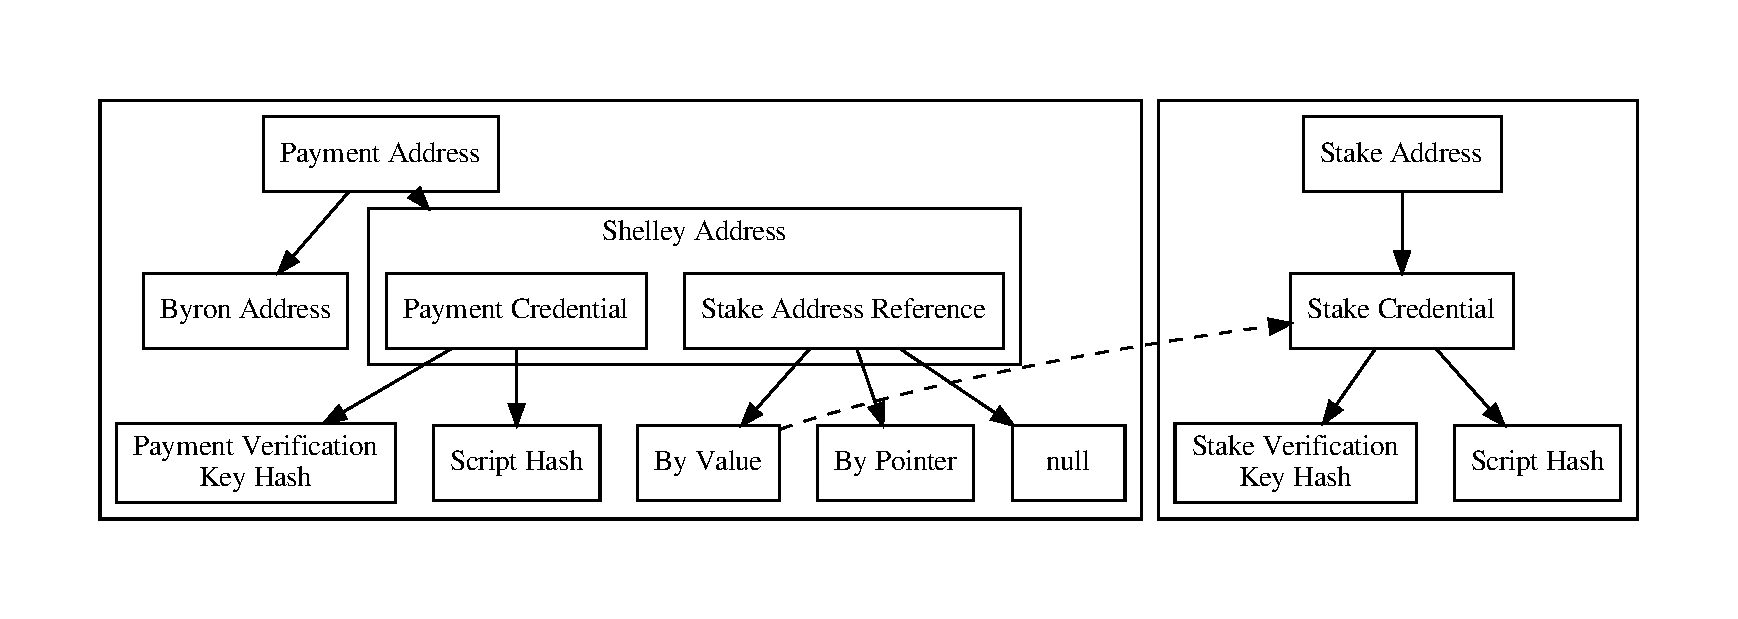
\includegraphics[width=\linewidth]{addresses.pdf}
  \caption{Addresses and Credentials}
  \label{fig:addresses}
\end{figure}

\cref{fig:addresses} shows the anatomy of both payment and stake addresses. Let
us first consider a \emph{Stake Address}: it contains a stake credential (which
can be a key credential or script credential). A stake address is used for two
purposes: delegating stake (see \cref{delegation-certificates}), and spending
rewards accumulated in a \emph{reward account} (see \cref{reward-accounts}).

\emph{Payment Addresses} have more structure: first of all, we have the two
cases of Byron and Shelley addresses. The purpose of Byron addresses is
backwards compatibility. Byron addresses have no notion of stake, so it is not
possible to delegate from a Byron address; users will have to transfer funds to
a Shelley address first.

A Shelley address contains a payment credential (again, either a key or script
credential). A transaction that consumes a UTxO entry with a Shelley address
will need a witness for this payment credential in order to be validated. In
addition, a Shelley address also contains a stake address reference. When
calculating the stake distribution (see \cref{delegation-relations} for
details), the system uses this reference to decide where to count the stake
corresponding to the tokens in this address.

There are three options for the stake address reference in a Shelley address: it
can be provided \emph{by value}, i.e., just be the hash of a verification key or
validator script. Shelley addresses that provide their stake address reference
by value are sometimes also called \emph{base addresses}.

There is also a more compact way of representing a stake address reference: since stake
addresses need to be registered on the chain in order to be considered for the
stake distribution (see \cref{stake-address-registration-certificates}), we can
also include them \emph{by pointer}, pointing to the certificate that
registered the stake address containing. Since the
blockchain orders transactions, this pointer is quite small, containing only
three numbers (slot index, transaction index within the block, and certificate
index within the transaction). Shelley addresses that contain their stake
 by pointer are also called \emph{pointer addresses}.

The third possibility is to not have a stake address reference at all. In this case,
the stake corresponding to the tokens in the address is not considered by the
system at all (just as for a Byron address). In particular, it will not be
counted towards the active stake (\cref{overall-stake-distribution}), and so
will not slow down chain growth. Users who do not wish to contribute to the PoS
protocol should use this option. Such addresses are also called \emph{enterprise
  addresses}.

\subsubsection{On Pointer Addresses}
\label{pointer-address}

Allowing the stake address reference to be included in a payment address via pointer
allows for shorter addresses, which is a requirement (\cref{short-addresses}).
However, there are also some subtleties to consider.

\paragraph{Invalid Refereces}
First, we need to consider the case that the pointer does not point to an
\emph{active} stake address registration. This covers the case that the key was
unregistered after (or indeed before) the transaction, and also covers pointers
to targets that are plainly invalid. The system will allow transactions to and
from such addresses, but their stake will not be considered for leader eleaction
and rewards.

Note that in particular, when a pointer address becomes invalid because the
stake address it points to is deregistered, registering the same stake address
again does not ``restore'' the stake in the pointer address; the tokens have to
be moved to another address in order to use the stake. This minor limitation
allows the system to not remember unregistered stake addresses.


So, to exercise the stake rights of a pointer address, the stake address must be
registered in advance of using the pointer address in the output of a
transaction, and the stake address must remain registered while the pointer
address holds funds. This is a difference compared to addresses that contain
their stake address reference by value, where the stake address can be registered
after the value address is used in a transaction.

\paragraph{Pointer Addresses and Rollback}
A special case of an invalid pointer is a rollback: when the block containing a
stake address registration certificate gets rolled back, addresses containing
the stake address by pointer to that certificate will lose their stake rights.
Since the addresses will remain valid for payments, though, the stake rights can
be restored by moving the funds to another address. Still, it is prudent to
avoid this, by either allowing a number of blocks between transactions \(t_1\)
registering a stake address and \(t_2\) moving funds to a pointer address for
this stake address, or by using an output of \(t_1\) as an input to \(t_2\).

\subsubsection{On Enterprise Address}
\label{enterprise-address}

Enterprise addresses carry no stake rights whatsoever and thus using
them allows completely opting out of participation in the proof of stake
protocol. Exchanges or other organisations that control large amounts of
ada -- but hold it on behalf of other users -- may wish to follow a
policy of not exercising stake rights. By using enterprise addresses,
exchanges can demonstrate that they follow this policy.
Since enterprise addresses are not associated with any stake address, they
are automatically excluded from the mechanisms that influence the slot
leadership schedule.

Note that using addresses with no stake rights effectively decreases
the total amount of stake, which plays into the hands of the adversary.
But unless we want the exchange to control the stake, it is unavoidable to
ignore it, since there is no way to determine whom the stake "really" belongs
to. Also note that it is generally considered bad practice to leave funds on
exchanges, and in Cardano-Shelley, there will also be a monetary incentive to
withdraw funds from exchanges in order to earn rewards.

\subsubsection{Reward Accounts}
\label{reward-address}

Reward accounts are used to distribute rewards for participating in
the PoS protocol (either directly or via delegation), as described in
\ref{distributing-rewards}. They have a number of interesting
properties:

\begin{itemize}
\item They use account-style accounting, not UTxO-style.
\item They can not receive funds via transactions. Instead, their
  balance is only increased when rewards are distributed.
\item A reward account is not related to a value address, but to a stake
  address. Thus, spending from a reward account requires a witness for a stake
  credential, rather than a payment credential.
\end{itemize}

Rewards can be ``withdrawn'' from a reward account, by using the reward account
as an input to a transaction. Note that we will still require at least one UTxO
style input in this transactions for replay protection, as explained in
\cref{certificate-replay-prevention}. Stake associated with funds in a reward
account will contribute to the stake of the stake address, so there is no
incentive to frequently withdraw rewards.

The terms \emph{reward address}, \emph{reward account}, and \emph{reward account
  address} will be used interchangeably throughout this document. \todo{Use
  reward account everywhere instead.}

\subsubsection{Byron Address}
\label{bootstrap-address}

In Byron, all addresses were interpreted as
having stake rights, but those stake rights were always delegated to a fixed set
of keys specified in the genesis block, controlled by the
Cardano Foundation, Emurgo, and IOHK.

Byron addresses continue to exist in Shelley, but their
interpretation is changed subtly and their use is disincentivised.
Their interpretation is changed from having stake rights with
forced delegation, to having no stake rights whatsoever. Their use is
disincentivised, since owners have the option to move their funds into
the new base or pointer addresses that have stake rights, which can be
exercised to receive rewards.

It is worth noting that initially, Byron addresses and enterprise addresses
have essentially identical behaviour. This might change in the future, if new
features are added to enterprise addresses.

\subsubsection{HD Wallet Structure in Shelley}
\label{hd-wallet-structure-in-shelley}

Shelley addresses with a verification key hash as payment credential
support hierarchical deterministic wallets, as per BIP-32~\citep{bip32}.

For multi-sig value addresses, we can use a slight generalisation of
BIP-45~\citep{bip45}\todo{Lay out the necessary generalisation of BIP-45}.

In particular, this kind of wallet scheme allows implementations that can
do wallet restoration from seed in time that is better than linear in
the total number of addresses in the blockchain. For details, see
\cref{wallet-recovery-process}.

\subsubsection{Address Recognition}
\label{address-recognition-1}

Wallets will recognise addresses (other than reward addresses) that belong to
them just as they would without delegation, by looking only at the
payment credential (see \cref{wallet-recovery-process} for how to find
addresses efficiently).

Finding the stake credentials of a wallet (and in particular the corresponding
reward accounts) can be done either by just reading off all the stake credentials
of addresses found via their payment credentials, or by performing a second search,
this time over all the registered stake addresses\footnote{As explained in
  \cref{stake-address-registration-certificates}, stake addresses need to be
  registered on-chain.}. The former option is quicker and easier to implement.
However, it is conceivable to construct addresses where the payment credential
belongs to one wallet, but the stake credential belongs to another. The stake
credential of such addresses would only be found by the wallet that controls it via
a dedicated search on the registered stake addresses.

Once a wallet recognises an address via its payment credential, it will read its
stake credential, and check whether it is set according
to the current delegation preference of the wallet. If there is a
discrepancy, it will alert the user, and ask them whether they want to
re-delegate according to their current delegation preferences.

This check protects against the malleability attack in
\cref{address-nonmalleability}. It does so not by making it impossible, but
by ensuring that the users are aware of it. This design also covers the case
of users simply changing their delegation choice but subsequently receiving
payments to addresses they handed out previously that use the previous
delegation choice.

\subsection{Certificates and Registrations}
\label{certificates-and-registrations}

\subsubsection{Certificates on the Blockchain}
\label{certificates-on-the-blockchain}

The registering of stake addresses and stake pools, and delegating
involves posting appropriate signed registration and delegation certificates to
the blockchain as part of the set of certificates included in
transactions. This makes the certificates part of
the blockchain, which means that they are are publicly announced to all
participants.

Certificates will remain valid
until explicitly overwritten or revoked, as an automatic expiry would
likely increase the amount of undelegated, offline stake. The following
certificates can be posted to the blockchain:
\begin{itemize}
\item Stake address registration certificate
\item Stake address de-registration certificate
\item Delegation certificate
\item Stake pool registration certificate
\item Stake pool retirement certificate
\end{itemize}
There is one form of certificate which is not posted to the blockchain
in advance, but is presented when it is used:
\begin{itemize}
\item
  Operational key certificate
\end{itemize}
Although this last kind is similar to delegation certificates in that
it uses one key to grant the right to sign blocks to another
key, it is quite different from the other certificates which are used
to define the delegation relation. Operational key certificates are
used by stake pool operators as a safety measure to mitigate key
theft (see \cref{operational-key-certificates}), not to delegate
staking rights between different entities.

Figure~\ref{fig:relationship-keys-certificates} shows the relationships between
the different types of certificates and keys.
%
Dashed arrows represent relationships between the different keys and addresses:
the owner(s) of a stake address delegates their staking rights to the owner of a
stake pool cold key, using a delegation certificate.
%
The owner of a cold and hot key grants the staking rights of their cold key to their
hot key, using an operational key certificate.
%
Incoming solid arrows represent the components of the delegation certificates.
So, for instance, a delegation certificate contains the stake address of the
delegator, and the (verifying part of) the stake pool key.
%
Subsequent sections provide more details.

\begin{figure}[ht]
  \centering
  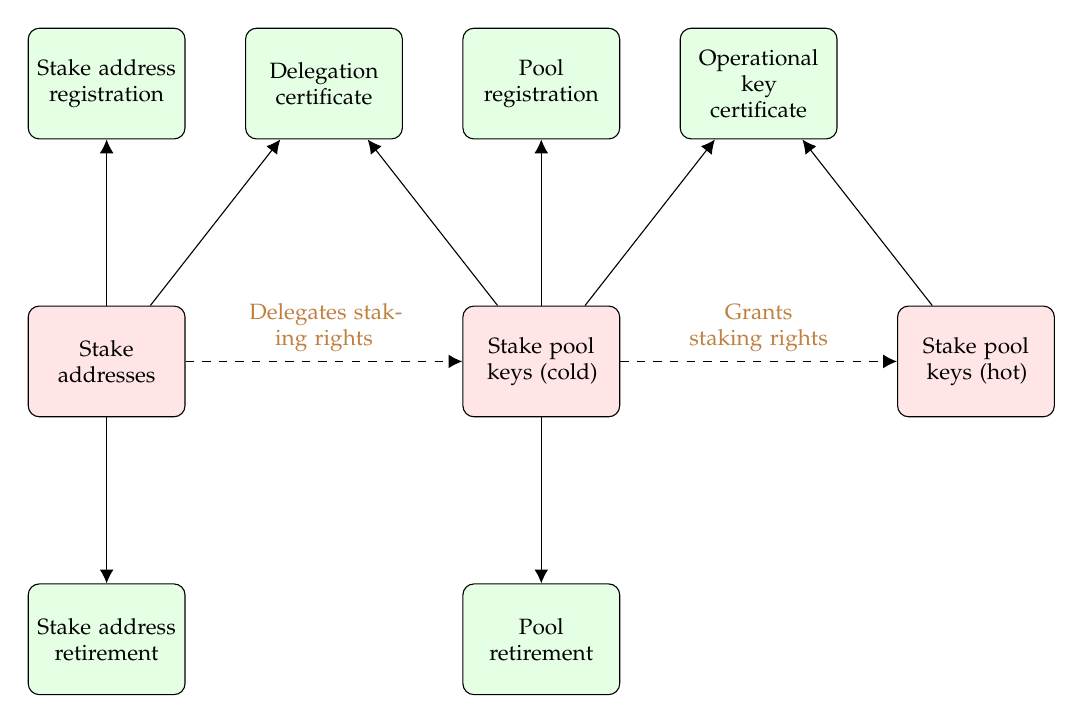
\begin{tikzpicture}[ align = center
                     , node distance = 6em and 10em
                     , text width = 5em
                     , font = \footnotesize
                     , >={Latex[width=0.5em, length=0.5em]}
                     , every node/.style = { rectangle
                                         , rounded corners
                                         , draw = black
                                         , align = center
                                         , minimum height = 4em }
                     ]

  %%
  %% Nodes
  %%
  \tikzset{ key/.style={fill=red!10}
          , cert/.style={fill=green!10}
          , dummy/.style={draw=none}
          }

  \node (skeys) [key] {Stake addresses};
  \node (scold) [key, right = of skeys] {Stake pool keys (cold)};
  \node (shot) [key, right = of scold] {Stake pool keys (hot)};
  \node (skeyr) [cert, above = of skeys] {Stake address registration};
  \node (skeyd) [cert, below = of skeys] {Stake address retirement};
  \node (pr) [cert, above = of scold] {Pool\\ registration};
  \node (pd) [cert, below = of scold] {Pool\\ retirement};
  \node (dcert) [cert] at ($(skeyr)!0.5!(pr)$) {Delegation certificate};
  \node (dummy) [dummy, above = of shot] {};
  \node (lwdcert) [cert] at ($(pr)!0.5!(dummy)$) {Operational key\\certificate};

  \tikzset{every node/.style={align=center, text width=7em, text=brown}}
  %%
  %% Relationship between nodes (arrows)
  %%
  % Horizontal lines.
  \draw[dashed, ->] (skeys) edge node[above] {Delegates staking rights}
  (scold);
  \draw[dashed, ->] (scold) edge node[above] {Grants\\ staking rights}
            (shot);
  % Vertical lines.
  \draw[->] (skeys) edge
            (skeyr);
  \draw[->] (skeys) edge
            (skeyd);
  \draw[->] (scold) edge
            (pr);
  \draw[->] (scold) edge
            (pd);
  \draw[->] (skeys) edge
            (dcert);
  \draw[->] (scold) edge
            (dcert);
  \draw[->] (scold) edge
            (lwdcert);
  \draw[->] (shot) edge
            (lwdcert);
  \end{tikzpicture}

  \caption{Relationships between the keys, addresses, and certificates}
  \label{fig:relationship-keys-certificates}
\end{figure}

\subsubsection{Certificate Replay Prevention}
\label{certificate-replay-prevention}

Unlike transactions, which inherently cannot be replayed due to the nature of
the UTxO accounting model, the certificates need an explicit mechanism to
prevent replays. The danger otherwise would include examples such as when a user
switches away from a stake pool by posting a new delegation certificate, the old
stake pool reposts the original delegation certificate, effectively thwarting
the user's attempt to delegate to another stake pool.

The solution we employ is to borrow an idea from UTxO witnesses and to
piggy-back on the inherent replay protection of the rest of the
transaction. A UTxO witness for an input is a signature on the entire
transaction body, which of course includes all inputs and outputs (but
not witnesses obviously). This means the signature can only be reused
on the same transaction, and due to the nature of UTxO accounting, the
same transaction cannot be included in the ledger again.

For certificates, we do essentially the same thing. The witness for a
certificate is a signature using the main key needed to authorise the
certificate (which is different for different kinds of certificate).
Just like UTxO witnesses, the witness is a signature on the entire
transaction body. This means that provided the transaction spends at
least one input then we inherit the inherent replay protection of UTxO
accounting. The validity rules for transactions will explicitly require each
transaction to have at least one UTxO entry as an input, so that certificates
will be protected from replay in this way.

Why do we need to explicitly state this requirement? Won't the need to pay
transaction fees always implicitly require a UTxO input anyway? There are two
additional sources of funds that could pay for the transaction fees: refunds and
the contents of a reward account. So it is possible to create transactions that
contain enough value to pay transaction fees even without consuming a UTxO
entry. Such a transaction, if valid, could be replayed at a later point in time.
In order to have all transactions (and by extension, all certificates), be
protected from replay attacks, we will explicitly require at least one UTxO
entry as an input to any transaction.

\subsubsection{Stake Address Registration Certificates}
\label{stake-address-registration-certificates}

Users wishing to exercise their rights of participation in the PoS protocol can
register a stake address by posting a \emph{stake address registration
  certificate} to the blockchain.

\begin{description}
\item[Stake address registration certificate] This certificate contains a stake
  address (see \cref{address-structure}), which can take the form of either a
  single key, or a multi-sig address.

  We do not require a witness to register a stake address (besides, of course,
  any witnesses needed for the transaction that is used to post the
  certificate).

We do not require a witness to register a stake key (besides, of course,
any witnesses needed for the transaction that is used to post the
certificate).

\item[Stake address de-registration certificate]
This certificate contains the stake address that should be de-registered.

The certificate requires a witness for the stake address that should be
de-registered. As stated in \cref{address-structure}, this will be a single key
or multi-sig witness, depending on the type of stake address in the certificate.

\end{description}

Registering a stake address introduces a corresponding reward account.
The account is deleted when the stake address is de-registered. See
\cref{reward-accounts-per-stake-key} for details on reward accounts.

In addition to a transaction fee, registering a stake address requires a
deposit, as explained in \cref{fees-deposits} and \cref{deposits}. The deposit
is to account for the costs of tracking the stake address and maintaining the
corresponding stake reward account. It also incentivises de-registering stake
addresses that are no longer required, so that the corresponding resources can
be released.

\subsubsection{Stake Pool Registration Certificates}
\label{stake-pool-registration-certificates}

A person planning to operate a stake pool (including a private pool) can
declare their intent by posting a \emph{stake pool registration certificate} to
the blockchain.

\begin{description}
\item[Stake pool Registration Certificate]
The certificate contains the following:

\begin{itemize}
\item
  The public key of the pool, \(vk_\text{pool}\).

\item
  A stake address \(\mathcal{A}_{s,\text{reward}}\), called the \emph{reward
    address} for the pool. Usually, this will be a \emph{registered} stake
  address, controlled by the pool operator. The rewards for the pool operator
  will be paid to the reward account of
  \(\mathcal{A}_{s,\text{reward}}\)\footnote{We do \emph{not} want to associate
    the reward account with the key of the pool itself. An important reason for
    this is that for security reasons, stake pool operators are required to use
    operational keys as described in \cref{operational-key-certificates}, while
    storing the key of the pool securely offline. Requiring the pool key for
    withdrawing rewards would be detrimental to this.}.

  If a pool operator wants to donate their rewards to a charity, they can do so
  by using a stake address that is controlled by that charity as the reward
  address. They can then advertise to other stakeholders that they are doing so
  (although evidence that the stake address does indeed belong to the charity
  has to be provided out of band).

  Should the reward address be unregistered, the stake pool operator will be
  unable to receive rewards. In that case, any rewards that they would be due
  are instead paid to the treasury (but the stake pool members would still get
  their usual rewards).

\item
  A list of stake addresses controlled by the pool owner(s),
  \(\mathcal{A}_{s,\text{owner}}\). If any of these \emph{owner stake addresses}
  delegate to this pool, the stake that they delegate will be counted towards
  the stake pledged to the pool by the owner(s), see
  \cref{stake-pool-registration,overview-of-incentives,reward-splitting}. Note
  that adding a stake address to the set of owner stake addresses in itself does
  not actually delegate the stake controlled by that address to the pool -- an
  additional delegation certificate is required to do so.

  During reward distribution, there will be no rewards paid to the reward
  accounts of the owner stake addresses. Instead, the stake delegated by all owner
  stake addresses will be counted as the stake contributed by the pool owner(s),
  and their reward will be paid to the reward account of the reward staking key.

\item
  The parameters that specify the reward sharing function of the stake
  pool: cost, margin, and amount of stake pledged to the pool by the
  owner(s), see \cref{stake-pool-registration,reminder-stake-pool-registration}.

\item
  A list of IP addresses and/or DNS Names of public relay nodes that the stake
  pool operator provides to support the Cardano network.

\item
  Optionally, a URL and content hash for additional metadata about the pool, for
  display in the wallet. The URL is restricted to a length of 64 bytes. It is
  the obligation of the stake pool operator that this URL points to a JSON
  object containing the metadata of the pool, as described in
  \cref{stake-pool-metadata}. The content hash of that JSON object should match
  the content hash in the registration certificate.

  If no URL and content hash is provided, the stake pool will not be listed in
  wallets. Private pools (\cref{individual-staking}) will use this option.

  Also, if there is a mismatch in the content hash, the pool will not be
  displayed. If a stake pool operator changes the metadata, they have to post a
  new stake pool registration certificate with the new content hash.
\end{itemize}

Validating the certificate requires witnesses from all owner stake addresses, as
well as a signature from the pool signing key \(sk_\text{pool}\)\todo{We could
  also just include the public pool key hash in the certificate, and have the
  key itself be provided in the witness, which would make the certificates a bit
  smaller. I think we should do that.}.

\end{description}

If a stake pool can foresee that it will cease to operate, it can
announce this intent by posting a \emph{stake pool retirement
certificate}.

\begin{description}
\item[Stake pool Retirement Certificate]
It contains

\begin{itemize}
\item
  The public key hash \(\mathcal{H}(vk_\text{pool})\) of the pool.
\item
  The epoch number, starting from which the stake pool will cease to
  operate.
\end{itemize}

It must be signed by the pool key \(sk_\text{pool}\) (particularly, it need not
be signed by any of the pool owners).

After the retirement epoch, any stake that is delegated to this stake
pool will be disregarded for the PoS protocol. It will not take part in
the leader election process (similarly to how stake in an enterprise
address is not considered during the election process).

Stakeholders who delegated to this pool should be notified and asked to
redelegate by their wallet the next time they are online.
\end{description}

\subsubsection{Single Operator, Possibly Multiple Owners}
\label{multiple-owners}

Note that there is a conceptual difference between the stake pool
\emph{operator} and stake pool \emph{owners}:
\begin{description}
\item[Stake Pool Operator] This is the person who operates the pool -- owns or
  rents a server, holds the key of the pool, runs and monitors the
  node.
\item[Stake Pool Owner] This is a person pledging stake
  to the pool, increasing its rewards and desirability. The ability
  for the owner to pledge stake is providing protection against the
  pool-level Sybil attack
  (requirement~\ref{sybil-attack-protection-at-stake-pool-level}, see
  also \cref{stake-pool-registration}).
\end{description}

Usually, the stake pool operator and owner will be the same person,
but a stake pool can also have multiple owners. This is to allow
people to coordinate and form a stake pool even if none of them had
enough stake on their own to make a pledge that would make the stake
pool competitive.

Still, there will only be one operator, the person holding the key of the stake
pool itself. In addition to signing blocks, this key also holds the power to
retire the stake pool, or to post updated registration certificates without the
keys of all owners (in which case some of the owners are kicked off the stake
pool). Also, the rewards for all owners will be paid to the reward account
associated with the reward address of the pool, and it will be the
responsibility of the person(s) owning that address (usually the pool operator) to
distribute the rewards amongst the owners.
That is a conscious design decision: collaborating to form a stake pool should
require significant trust between the owners. Otherwise, everyone could choose
to become a co-owner of a stake pool instead of delegating, which would render
the mechanism of pledging stake ineffective. Allowing the operator to shut down
the pool, kick other owners off, or fail to distribute rewards raises the
threshold of necessary trust that owners of the pool must have in the operator.

\subsubsection{Delegation Certificates}
\label{delegation-certificates}

Users can transfer the rights of participation in the PoS protocol from
their stake address to a stake pool, by posting a \emph{delegation
certificate} to the blockchain.

\begin{description}
\item[Delegation Certificate]
A delegation certificate is a tuple containing

\begin{itemize}
\item
  the stake address delegating its staking rights,
  \(\mathcal{A}{s,_\text{source}}\)
\item
  the public stake pool key hash to which stake is delegated,
  \(\mathcal{H}(vk_\text{pool})\)
\end{itemize}

Posting a delegation certificate requires a witness for
\(\mathcal{A}{s,_\text{source}}\).
\end{description}

Note that there is no corresponding delegation revocation certificate.
If a user wishes to change their delegation choice to a different stake
pool or their own private stake pool then they can simply post a new
delegation certificate. The delegation certificate is revoked when the
source staking key is de-registered.

\subsubsection{Operational Key Certificates}
\label{operational-key-certificates}

% On the need for a hot/cold key arrangement.
Stake pool operators must use a \emph{hot}/\emph{cold} key
arrangement to mitigate key exposure
(see~\cref{mitigate-key-exposure}). A \emph{hot}, or operational, key
is kept online and used to sign blocks, while the \emph{cold} key is
kept securely offline. This requires an \emph{operational key
  certificate} to create a (1-link) chain of trust from the cold key
to the hot key, allowing this hot key to participate in the \emph{PoS}
protocol. Should the hot key become compromised, the stake pool
operator should immediately create a new operational key certificate, and
switch to a new key.

% The problems with using in-ledger certificates.
If the operational key certificates would be included in the ledger,
as the other certificates are, this would present a problem for block
validation. Consider the following example: suppose that the network
layer wants to validate a batch of 10 block headers from the current
epoch, before deciding if it wants to also download the block
bodies. Can it tell if those block headers are signed by the right
actors?

In this situation the network layer has the state of the ledger up to
but not including these next 10 block headers. So it cannot rely on
any information in the 10 corresponding block bodies.

Without this information, the validity of the hot key that signed
the headers cannot be verified. If the network layer sees one of the
10 new blocks signed by a hot key it doesn't recognise, it might be
because there is a delegation certificate in the block bodies (which
the network layer has not seen yet), that shows that the key is valid
because some stake pool key deferred its staking rights to it. Similarly,
if the network layer sees a known hot key, how can it know that it
is still valid? There could be a new certificate in the block bodies
that defers the rights of this key to a different one (which would
invalidate the key the network layer saw).

To address this problem, a new type of certificate is introduced:
\emph{operational key certificates}. These certificates are provided
in the block header itself, as part of the witness, thus solving the
problem of determining the validity of hot keys. In other words,
operational key certificates are \textbf{not included in
  the ledger}, but instead they are \textbf{included in a witness} by
stake pools at the point of exercising stake rights including:

\begin{itemize}
\item
  signing blocks
\item signing votes for protocol update proposals (once the update and
  voting system is in place)
\end{itemize}

An operational key certificate, signed by the stake pool's cold key,
delegates to the hot key that is used to sign messages in the
protocols (block header or vote). This operational key certificate is
included in the message so that all other nodes can verify that the
message is signed by a legitimate delegate of the owner of the cold
key\footnote{This is much the same setup as with TLS certificates:
  there are known root certificates, but the server's operational
  certificate is presented inband.}.

Specifically, an operational key certificate specifies that the
staking rights are transferred from a cold stake poo key \(vk_\text{pool}\)
to a hot key \(vk_\text{hot}\).
They are included in the message (e.g.~block header) and the message
itself is signed with \(sk_\text{hot}\).

Operational keys will use key evolving signatures (KES). To be precise, we will
use keys according to the MMM scheme \citep{cryptoeprint:2001:034}, regular
evolutions after a number of slots that correspond to one day, and a key
lifetime of \(2^7 = 128\) days, a little over three months.

Operational key certificates will have a lifetime of 90 days after which they
become invalid, to encourage pool operators to regularly rotate their
operational key. The certificate will specify a slot from which it will be
considered to be valid for 90 days.

In detail, the hot/cold key setup is as follows:

\begin{itemize}
\item
  The stake pool operator registers their stake pool, using a cold stake pool key
  \(vk_\text{pool}\). This \emph{cold key} is kept securely and
  off-line.
\item The stake pool operator uses \(sk_\text{pool}\)
  to sign an operational key certificate \(C\),
  transferring the staking rights to a \emph{hot key}
  \(vk_\text{hot}\).
\item
  The stake pool operator keeps \(sk_\text{hot}\), as well as \(C\), on
  a node that is on-line, and can sign blocks. A block signed with
  \(sk_\text{hot}\) will be considered valid, provided that \(C\) is
  included in its header.
\item
  Should the node get hacked, and the hot key compromised, the stake
  pool operator will create a new operational key certificate
  \(C'\), delegating the staking rights to a new hot key
  \(vk_{\text{hot}'}\).
\end{itemize}

In order to render \(sk_\text{hot}\) useless, it must be established
that \(C'\) takes precedence over \(C\). For this purpose, the
operational key certificate will have an additional integer
field, and certificates with a larger value for this field will take
precedence.

\subsubsection{Certificate Precedence and Validity}
\label{certificate-precedence-and-validity}

The following rules determine precedence and validity of certificates.
In particular, they describe what happens when multiple certificates are
issued for a given stake pool key.

The ordering of blocks and transactions induces a canonical ordering
amongst certificates. Thus, the terms older/newer certificate are well
defined and are used below.

\paragraph{Stake Pool Registration and Retirement Certificates}

\begin{itemize}
\item
  There can be at most one active stake pool registration certificate
  for any given stake pool key. A newer certificate will override an older
  one.

  This will allow stake pool operators to update their costs and margin
  if they need to\footnote{Stake pool members should be notified of such changes
  by their wallet the next time they are online, if this makes the pool less
  desirable, see \cref{display-of-stake-pools-in-the-wallet}.}.
\item
  A revocation certificate is only valid if there is an older
  registration certificate.
\end{itemize}

\paragraph{Delegation Certificates}

Newer delegation certificates override older delegation certificates. This
allows delegators to move from one stake pool to another.

\paragraph{Operational Key Certificates}

For operational key certificates, we cannot rely on the ordering induced by
the blockchain. But we do have the counter field, which serves the
purpose of establishing precedence:

\begin{itemize}
\item
  An operational key certificate with a higher counter overrides one with a
  lower counter.
\item
  Also, we require that within any given chain, if there are two blocks A and B
  signed using operational key certificates issued by the same cold key, if A is
  an older block than B, the counter in the operational certificate in the cert
  in the header of B must be at least as large as the one in the counter in the
  operational certificate in the header of A.
\end{itemize}

\subsection{Delegation Relations}
\label{delegation-relations}

As stated in the delegation overview: delegating stake rights involves
two indirections: from addresses to stake addresses, and from stake addresses to
stake pools.

Equivalently, there are two relations: a relation between addresses and
stake addresses, and a relation between stake addresses and stake pools. The base
and pointer addresses form the entries of the first relation. The second
relation consists of registered stake addresses, registered stake pools and
delegation certificates as the entries relating the two.

\subsubsection{Address Delegation Relation}
\label{address-delegation-relation}

The address delegation relation is a relation between addresses and
stake addresses.

This relation can be defined in terms of the current UTxO and the
current set of registered stake addresses. For all base addresses in the
UTxO, the stake address is given directly, so this need only be
filtered by the current set of registered stake addresses. For pointer
addresses in the UTxO we select those where their pointer points to a
currently registered stake address and select this stake address.

\subsubsection{Stake Pool Delegation Relation}
\label{stake-pool-delegation-relation}

The stake pool delegation relation is a relation between stake addresses and
stake pools.

The relation is defined by the active set of delegation certificates,
filtered by the set of active stake pools. The active delegation
certificates already excludes those where the source stake address has
been de-registered.

\subsubsection{Overall Stake Distribution}
\label{overall-stake-distribution}

Ouroboros \citep{ouroboros_classic} requires a stake distribution to
use as the basis of defining the slot leader schedule for the next
epoch.

The overall stake distribution is the set of all registered stake pools
and their aggregate stake from all addresses that are delegated to them.

This can be defined by taking the composition of the address delegation
relation and the stake pool delegation relation, giving the relation
between addresses and stake pools. The final distribution is formed by
taking the transaction outputs from the UTxO and selecting all the
addresses related to each stake pool and aggregating all the coins.

Note that defining the stake distribution in this way is in contrast to
using the follow the Satoshi algorithm. This definition automatically
excludes all addresses that hold no stake, and excludes addresses with
stake rights but that have not correctly registered their staking key or
delegation choice.

We will call stake that is correctly delegated to an existing pool \emph{active
  stake}, sometimes contrasted to the \emph{total stake}, which includes stake
that is not delegated (or delegated to pools that are already retired).

\subsubsection{Chain Delegation}
\label{chain-delegation}

Chain delegation is the notion of having multiple certificates chained
together, so that the source key of one certificate is the delegate key
of the previous one.

While the delegation research paper in principle allows a significant
degree of flexibility with delegation, our chosen design is quite
restrictive and uses a fixed pattern of delegation.

We will only allow a very simple form of chain delegation, where we have
the following, in order:

\begin{enumerate}
\item
  a stake address
\item
  a delegation certificate; and
\item
  an operational key certificate.
\end{enumerate}

This restricted pattern of chain delegation allows us to satisfy all
requirements, but avoids problematic cycles in the graph of delegation
certificates, and makes it simple for nodes to track the delegation.

\subsection{State Tracking for delegation}
\label{state-tracking-for-delegation}

It is not sufficient for certificates to be posted to the blockchain.
Nodes need ready access to certain parts of previously posted
information as part of the protocol execution or ledger validation. For
example, since nodes need to validate signatures on new blocks in a
timely manner, they need ready access to information about the registered
stake pools (including operational key certificate validity).

One of the design goals is to avoid having to look up old entries on the
blockchain, since we want to allow implementations that forget old
blocks. Instead, we want a {\tt foldl} design where nodes keep track -- as
local state -- of all the information they will later need.

The following sections describe the local state that nodes must maintain
as they process transactions in blocks.

\subsubsection{Staking Keys}
\label{stake-keys}

The set of active staking keys must be tracked. This contains the
verification key \(vks\) from each staking key registration certificate.
The set is uniquely indexed by the key hash \(\mathcal{H}(vks)\). It is
also uniquely indexed by the location on the blockchain of the key
registration certificate, using the same location type as pointer
addresses.

This set is updated when keys are registered and de-registered. This
state is consulted when validating and applying transactions that
withdraw from reward accounts, to retrieve the staking key for a reward
account address.

\subsubsection{Reward Accounts}
\label{reward-accounts}

For each staking key there is an associated reward account. The lifetime of
these accounts follows exactly their associated registered staking key.

The reward accounts are a mapping from a reward account address to
their current balance. This address is the unique index for the mapping.
The staking key account address is a function of the associated key hash
\(\mathcal{H}(vks)\), as described in \cref{reward-address}.

The accounts are updated in bulk following the end of an epoch. They are
consulted and updated when validating and applying transactions that
withdraw from reward accounts. See \cref{distributing-rewards} for
details.

\subsubsection{Stake Pools}
\label{stake-pools}

The set of active stake pools must be tracked, uniquely indexed
by the public key hash of the stake pool.

In addition, a small amount of state needs to be maintained to validate
operational key certificates. The state tracked for each stake pool includes
an integer representing the highest counter field seen so far in a valid
certificate. This is consulted to validate operational key certificates, and
updated when larger counter values are presented in a valid certificate.

\subsubsection{Active Delegation Certificates}
\label{active-delegation-certificates}

Active delegation certificates are tracked, as a finite map from
source to target staking key hash.

\subsubsection{Stake per Staking Key}
\label{stake-per-staking-key}

For the purpose of leader election and reward calculation, the system
needs to know how much stake each registered and delegating staking key
actually controls. The total stake is calculated as the sum of all
funds that are
\begin{itemize}
\item in base addresses using that staking key
\item in pointer addresses for that staking key's registration
  certificate (as long as the requirements in \cref{pointer-address} are
  fulfilled)
\item in the reward account of that staking key
\end{itemize}

\subsection{Slot Leader Schedule and Rewards Calculation}
\label{slot-leader-schedule}

The process of leader election has to be modified to take delegation
into account.

While adding blocks to their chain, nodes will keep track of the
pieces of state listed above. When it is time to prepare the slot
leader schedule for the upcoming epoch, they will look at a past
snapshot of that state, from slot \(s_\text{stakedist}\), the slot
from which the stake distribution should be used to compute the slot
leader schedule and rewards for the next epoch\footnote{The detail of
  which slot is used as \(s_\text{stakedist}\) depends on the variant
  of the Ouroboros protocol that is used. It needs to be deep enough
  in the chain to be stable. It also needs to be before the point in
  time at which the random seed for the slot leader election is
  determined, to prevent a grinding-type of attack. Note that
  \(s_\text{stakedist}\) does not necessarily have to be in the
  current epoch.}.

The nodes will use the state from slot \(s_\text{stakedist}\) to
\begin{itemize}
\item compute the stake distribution (i.e., the amount of stake per
  stake pool)
\item create the leader schedule by sampling the stake distribution
  (i.e., sampling the stake pools, weighted by the stake they control)
\item retain this state, to use it for the reward calculation at the
  end of the epoch\footnote{They cannot calculate those rewards
    immediately, because they depend on the efficiency of the pools
    during the following epoch. However, they could, alternatively to
    retaining the whole delegation state, calculate the rewards up to
    the factor that depends on the efficiency.}.
\end{itemize}

\subsection{Block Validity and Operational Key Certificates}
\label{block-validity-and-operational-key-certificates}

Stake pool operators will use operational key certificates in order to protect
the key to which their members delegated. A block for a slot where the key
\(vks_\text{leader}\) has been elected as leader will be considered valid by all
nodes if

\begin{itemize}
\item
  the block is signed by \(vks_\text{hot}\) and contains, in its header, an
  operational key certificate that transfers the staking rights from
  \(vks_\text{leader}\) to \(vks_\text{hot}\).

\item
  The counter of the operational key certificate must not be smaller than the
  counter of the operational key certificate used to sign the last block of
  \(vks_\text{leader}\).
\end{itemize}

In case there are more than one block for the current slot, each of
which are signed using an operational key certificate, the newest certificate
(as per the included counter) takes precedence.

Note that nodes take the precedence amongst operational key certificates into
account only \emph{after} comparing the length of the chains. When the node is
already up to date and receives two conflicting blocks that add to its current
chain, the length will of course always be the same. But this rule is important:
if we did not compare the lengths of the chains before giving preference to the
block with the newer operational certificate, it would be possible to force a
node to do a rollback of arbitrary length, by sending it a block from a past
slot, signed using a newer certificate than the block that the node already has
in its chain for that slot. This would open up an attack where a stake pool
operator could force nodes to do arbitrary rollbacks.

\subsection{Transition to Decentralization}
\label{transition-to-decentralization}

In order to guarantee system stability, we must be sure that stake pool
operators are ``doing their job'' sufficiently well before relinquishing
control to them. Instead of having a simple ``switch'' from a
centralized system controlled by a handful of bootstrap keys to a fully
decentralized one, we propose a \emph{transition phase}.

\subsubsection{Motivation}
\label{motivation}

Cardano \emph{chain growth quality} is only guaranteed when for all time windows
of \(2k\) slots, a block has been created for at least \(k\) slots, where \(k\)
is the security parameter of the protocol. At the moment, the bootstrap nodes
are responsible for block creation, but in a fully decentralized system, this
will be the pool operators' responsibility.

In the beginning, there might be technical problems or other issues
preventing the pool leaders from creating sufficiently many blocks, so
we want to make the transition gradual, monitoring system performance
and being able to temporarily delay or even revert decentralization in
case of an emergency.

Another consideration is the amount of stake that is necessary to mount
a 51\% attack on the system. Since participating in the PoS protocol
requires an action on behalf of the stakeholders -- registering their
staking key and delegating -- it is not unreasonable to expect that it
will take some time until a significant fraction of the overall stake
becomes active and starts contributing to the protocol. An attacker
might use this window of opportunity to attack the system. A gradual
handover of the protocol from the initial core nodes to the actual
stakeholders will protect the integrity of the blockchain.

\subsubsection{Proposal}
\label{proposal}

We propose to introduce a new parameter \(d\in[0,1]\), which controls
the ratio of slots created by the bootstrap keys -- all other slots will
follow the rules outlined in this specification. So \(d=1\) corresponds
to the present ``bootstrap era'' state, whereas \(d=0\) corresponds to
full decentralization as described in this document. Starting with
\(d=1\) and gradually going down to \(d=0\) allows for a smooth
transition period.

For a given value of \(d\), the system will perform two steps to create the
leader schedule for the next epoch:
\begin{itemize}
\item Perform leader election amongst the new nodes, according to Ouroboros
  Praos, for all \(n_s\) slots in the epoch.
\item Randomly select \(d n_s\) slots of the epoch. Let us call those the slots
  the \emph{OBFT slots} of that epoch. For the OBFT slots, the Praos leader
  schedule will be overridden, and the old core nodes will be responsible for
  creating blocks for theses slots.

  In order to keep the block frequency constant, we will select a fraction
  \(f\) of the OBFT slots, where \(f\) is the active slots coefficient from
  Praos\footnote{In Ouroboros Praos, a large fraction of slots will deliberately
  be empty, which makes it easier to treat network delays in the adversarial
  model, and to still give guarantees of liveness and persistence when some
  blocks are not propagated within a single slot. Note that it is still possible
  to achieve the same block frequency as in Ouroboros Classic, by choosing a
  shorter slot length.} (Equation (1) in \citep{ouroboros_praos}), and call
  those the \emph{active OBFT slots} of the epoch.

  For OBFT slots, we will modify the behaviour of all nodes as follows:
  \begin{itemize}
  \item
    No stake pool node shall create a block for an OBFT slot.
  \item
    For non-active OBFT slots, no node shall produce a block at all -- neither
    one of the old core nodes, nor one a stake pool node.
  \item
    Also, for the non-active OBFT slots, no block shall be considered valid by
    any node.
  \item For the active OBFT slots, the old core nodes will create blocks, in a
    round-robin fashion as per OBFT.
  \item
    Blocks produced according to this schedule for the active OBFT slots shall
    be considered valid by all nodes.
  \end{itemize}
\end{itemize}

\subsubsection{Rewards during the Transition Phase}
\label{rewards-during-the-transition-phase}

We do this soft transition as a de-risking strategy, so that we can intervene in
case we observe any difficulties in the decentralised system. But we do not want
this to have an effect on the rewards that pools get. Operational difficulties
of the overall system that cause us to slow down the transition should not
reduce the rewards that individual pools get.

In order to minimise the influence of the transition on pool rewards, we have to
alter the way we measure the apparent performance for pools (see
\cref{stake-performance-and-block-production}) during the transition phase:
\begin{enumerate}
  \item
    For determining the apparent performance of any pool, we will take the total
    number of blocks in the epoch -- \(\Nbar\) in \cref{eq:beta} -- to be the
    number of blocks produced in \emph{non-OBFT slots}.
  \item
    As long as we have \(d >= 0.8\), we set the apparent performance of any pool
    to \(1\).
    \label{item:perf1}
\end{enumerate}
The reason for \cref{item:perf1} is that when only a small fraction of blocks
are produced by stake pools, the measurement of the performance will be
dominated by the statistical aspect of the leader election, and pools might
frequently get a performance of \(0\) by no fault of their own.

As an example\footnote{In this example, we assume \(n_s*f=21600\), to match the
  block frequency of Byron.}, consider a pool \(A\) with 1\% of stake. In the
fully decentralized case \(d=0\), \(A\) would be elected slot leader for
\(0.01\cdot 21600=216\) slots per epoch on average. For \(d=0.9\), \(A\) would
only be elected for \(0.01\cdot 0.1\cdot 21600=21.6\) slots per epoch on
average, so \(A\) would only have a tenth of the work (create 21.6 blocks
instead of 216 blocks), but get the same rewards.

\subsubsection{Transition Plan}
\label{transition-plan}

The parameter \(d\) can be changed on an epoch-per-epoch basis, following
the plan we will outline.

We plan to start with \(d=0.9\) and then decrease \(d\) by \(0.1\) each
epoch, \emph{provided pool leader block creation is sufficient to
guarantee chain growth quality, and a sufficient fraction of active
stake}.

If block creation is insufficient, we will halt lowering \(d\) (or even
increase \(d\) again) until we have reason to believe that the problem
has been understood and fixed.

In order to decide whether block creation is sufficient, we will
estimate the probability that at least \(k\) out of every \(2k\) blocks
would be created. If this probability is high enough (for example
greater than \(1 - 10^{-10}\)), block creation will be deemed
sufficient.

For the estimation, we use the
\href{https://en.wikipedia.org/wiki/Beta-binomial_distribution}{Beta-Binomial
Distribution}: Given the number of slots \(a\) that have been faithfully
created and the number \(b\) of slots that have been missed (counting
from the beginning of the transition period) and using
\href{https://en.wikipedia.org/wiki/Beta_distribution\#Bayes'_prior_probability_(Beta(1,1))}{Bayes'
Prior \(B(1,1)\)}, the probability in question is \(P(X\geq k)\),
where \(X\) is drawn from the Beta-Binomial distribution with parameters
\((a + 1)\), \((b + 1)\) and \(2k\).

For example, in the very first transitional epoch, 10\% of active slots,
i.e.~2160 active slots\footnote{assuming \(k=2160\) and an epoch length of
  \(10k\) active slots, as in Byron} will be given to pool leaders. If at least
1261 out of these 2160 slots are properly created, above estimation (with
\(a\geq 1261\) and \(b\leq 2160-1261=899\)) leads to \(P(X\geq 2160)\geq
1-10^{-10}\), so we will proceed with \(d=0.8\) in the second epoch. If however
at least 900 slots are missed, we will keep \(d\) at \(0.9\) for the time being.

In addition to monitoring the number of missed blocks, we will also look
at the fraction of stake that is active (i.e., is stored in addresses
which belong to a registered staking key that is delegating to a stake
pool). The lower this ratio, the less stake is required to launch a 51\%
attack on the system. This can be offset by increasing \(d\). For
example, if \(d \geq 0.5\), it is impossible to launch a 51\% attack. We
can specify an amount of stake controlled by an adversary that we want
the system to be resilient against, and delay reducing \(d\) in order to
meet this level of resistance.

\subsection{Rewards}
\label{rewards}

For the smooth operation of the system, it is beneficial to have a large
portion of the stake delegated to a set of reliable stake pools. Thus,
we should incentivise delegating stake to reliable stake pools. One way
to do this is to have stake pools share their rewards with their
participants.

The reward sharing mechanism should satisfy the following requirements:

\begin{enumerate}
\item
  Sharing rewards should be an automatic process that does not require
  an action, neither by the stake pool operator nor the participants.
  This requirement is not only meant to ensure that participants get
  their share reliably. The share of the rewards that are given to a
  particular participant depends on the amount of stake that that
  participant delegated in a particular epoch. Thus, any node that
  verifies a transaction that transfers the rewards for a given epoch
  needs to access the staking information for that epoch. While this
  information is archived on the blockchain indefinitely, looking it up
  for arbitrary past epochs might be too costly. Making the sharing of
  rewards an automatic process in the following epoch circumvents this
  problem.
\item
  Sharing rewards should not lead to an excessive growth of the UTxO. In
  particular, it should avoid creating dust entries.
\item
  Sharing rewards should not lead to a burst of transactions that risks
  pushing the system to the limits of its predictable region of
  operation.
\item\label{rewards-requirement-linkability}
  Sharing rewards should not increase the linkability of addresses of a
  wallet.
\item
  The reward sharing policy of the stake pool should be transparent to
  potential participants.
\end{enumerate}

Coming up with a solution that satisfies all of those requirements is
less straightforward than one might think. We did an exhaustive
assessment of possible approaches, documented in
\cref{assessment-of-rewards-sharing-mechanisms}, and finally opted for
the mechanism described in~\ref{reward-accounts-per-stake-key}, which
compromises somewhat on \cref{rewards-requirement-linkability}, but
satisfies all the other requirements.

\subsubsection{Distributing Rewards}
\label{distributing-rewards}

One of the difficult problems we had to solve during the design of the
reward distribution mechanism was UTxO explosion and dust creation:
since rewards occur in every epoch, and all the entries in the UTxO
will generate rewards, a naive approach would lead to an exponential
growth of the UTxO, which is clearly not sustainable. Furthermore,
individual rewards would be small, so most of the UTxO entries created
for reward distribution would be dust.

We have explored several approaches to circumvent this problem
(see \cref{assessment-of-rewards-sharing-mechanisms} for a summary),
and ended up with using \emph{reward accounts}
(\cref{reward-address}). Here, UTxO growth is prevented by using
addresses that do not use UTxO style accounting at all. Instead, every
registered staking key has an associated address that uses
account-style book-keeping. That way, the rewards from multiple epochs
can be pooled, and stakeholders can withdraw them manually. Note that
this has two advantages over the superficially simpler approach of
having stakeholders claim their rewards directly:
\begin{itemize}
\item Updating the total rewards a stakeholder is due happens
  frequently, avoiding the need for all nodes to hold on to the state
  that is needed to calculate rewards from old epochs.
\item Rewards that are accumulated in reward accounts can be used for
  staking before it is withdrawn, eliminating an incentive for
  frequent withdrawals (which again would lead to an unnecessary
  growth of the UTxO set).
\end{itemize}

After the end of each epoch, rewards for stake pool operators and members are
calculated, using the formulae in \cref{non-myopic-utility}. The calculation
will be based on
\begin{itemize}
\item The active stake pools, in particular their cost and margin parameters,
  pledged stake, owner key hashes, and reward accounts for stake pool owners.
\item The finite map giving the total stake for each registered
  staking key, \emph{taken at the point in time that was relevant for
    creating the leader schedule for that epoch}.
\item The stake pool delegation relation.
\item The leader schedule and list of empty slots for that epoch.
\end{itemize}
For each registered staking key, the rewards thus calculated are added
to the balance of the associated reward account.

Note that all the information that is relevant for the calculation of
the rewards is publicly available on the blockchain, so there is no
need to explicitly write the balance of each reward account to the
chain. Instead, it suffices for all the nodes to store the reward
accounts and their current balance locally.

\paragraph{Collecting Rewards}

Once a sizeable amount of funds has accumulated in a given reward
account, the owner of that account will want to withdraw those funds,
and move them to an ordinary address of their wallet. This withdrawal
from an account to a UTxO can be done via a special transaction. It
needs to be signed by the staking key the account belongs to.

The transaction is protected against replay by the requirement of having at
least one UTxO input, as described in \cref{certificate-replay-prevention}.

\paragraph{Handling of Bootstrap Addresses}
\label{handling-of-bootstrap-addresses}

All funds in bootstrap addresses will be ignored by the PoS system --
there is no staking key associated with bootstrap
addresses. Consequently, there will be no rewards, and stakeholders
will be incentivised to stop using bootstrap addresses. Our transition
plan, laid out in \cref{transition-to-decentralization}, prevents a
situation where the system would be vulnerable to a 51\% attack
because only a small fraction of the total stake is active yet, by
allowing for a period where the original nodes from the bootstrap
phase are still eligible to sign some of the blocks.

\subsection{Fees}
\label{fees}

To prevent economic attacks, fees or refundable deposits should be
charged where operators incur costs. In particular we will have
refundable deposits corresponding to the state that has to be tracked
for certificates\footnote{We plan to extend this to also cover UTxO entries in
  the future.}.

\subsubsection{Transaction fees}
\label{transaction-fees}

The basic transaction fee covers the cost of processing and storage. The
formula is

\(a + b x\)

With constants \(a\) and \(b\), and \(x\) as the transaction size in
bytes.

The fixed component is to cover per-transaction overheads. The component
linear in the size of the transaction reflects the processing and
storage cost of transactions.

This aspect remains unchanged with delegation except to the extent that
there are additional objects that can appear in transactions relating to
delegation. These simply increase the size of the transaction and so are
covered by the existing fee formula.

In principle different fees could be charged for different things
appearing in a transaction, to reflect their different processing costs.
This is a future direction, but will not be introduced as part of
delegation.

\subsubsection{Deposits}
\label{fees-deposits}

In addition to ordinary (non-refundable) fees, actions that require
resources on the nodes should require a deposit, as described in
\cref{deposits}. In particular,
\begin{itemize}
\item registering a staking key
\item registering a new stake pool (but not updating the registration
  certificate of a stake pool that already exists)
\item creating a new UTxO entry (in a future release)
\end{itemize}
should all require making a deposit. This deposit should be released
when
\begin{itemize}
\item a staking key is de-registered
\item a stake pool is retired -- there is a subtlety here, however,
  since the retirement certificate states an epoch in the future where
  the pool will cease operation. The refund should depend on that
  epoch, and we will delay paying out the refund until that epoch.
\item a UTxO entry is removed by using it as an input to a transaction (in a
  future release)
\end{itemize}
Note that posting a delegation certificate does \emph{not} require a
deposit; delegation certificates need a staking key registration
certificate in order to be valid, so any deposit that we would require
for a delegation certificate can instead be included in the deposit
for the associated staking key registration certificate.

\subsection{Time to Live for Transactions}
\label{time-to-live-for-transactions}

For multiple reasons, we will require that transactions that are submitted to
the system include a \emph{Time to Live} (ttl), a slot number\footnote{We use
  the term ``slot number'' to refer to an absolute slot number, i.e., specifying
  both the epoch and the slot throughout this document.} after which the
transaction can not be included in the ledger any more. An obvious advantage is
that this gives users the certainty that a transaction that failed to be added
to the chain can not be replayed in the future, so that they are safe to re-send
funds.

In the context of deposits and refunds, a ttl also proves to be useful: When a
transaction that releases a resource is created and submitted, it is not known
when it will be effective, and thus the refundable part of the deposit -- which
depends on the time at which the resource is freed -- can not be computed. But
if the transaction does include a ttl, the latest slot in which the transaction
can be added to the ledger can be used to calculate the refund.

\subsection{Robustness at the Epoch Boundary}
\label{robustness-at-the-epoch-boundary}

As described, there is a lot of work to be done by the nodes as the system
progresses from epoch to epoch: the stake distribution and slot leader schedule
need to be calculated, the fees accumulated during the epoch need to be
summed up, performance of the pools evaluated, deposits decayed, and
rewards determined and distributed.

Doing all that \emph{at} the transition between two epochs is far from ideal. It
creates a time period where all the nodes will need additional resources. It
also requires that all nodes finish those calculations within a single slot
length, and failure to do so will result in missed blocks and temporary forks.
Worse, since this period of increased activity is perfectly predictable, any
attacker of the system can leverage this, and time their attack appropriately to
maximise impact. Effectively, a predetermined breaking point is introduced at
the epoch boundary.

It is thus desirable to spread this work out over a longer period when possible.
And it turns out that this is entirely achievable.

\subsubsection{Calculating the Leader Schedule}

The stake distribution and randomness used to determine the leader schedule for
epoch \(e\) need to be available at the start of epoch \(e\). In the case of a
public leader schedule, it is also convenient to publish the schedule itself at
the start of the epoch. But we can start calculating those \emph{before} the end
of epoch \(e-1\). The details of when the stake distribution has to be taken for
the leader election, and when the randomness has to be agreed on, depends on the
choice of consensus protocol.

\subsubsection{Calculating and Distributing Rewards}

The rewards for epoch \(e\) depend on the contents of that epoch, so it is not
feasible to start calculating them during that epoch. However, there is no hard
constraint to actually distribute those rewards at the beginning of epoch
\(e+1\). If we instead defer that payout by one epoch, and pay rewards for epoch
\(e\) at the beginning of \(e+2\), we will have a whole epoch for that
calculation.

\subsection{Wallet Recovery Process}
\label{wallet-recovery-process}

Wallet recovery is the process of reconstructing a wallet from the root
key. In order to reconstruct a wallet, all addresses belonging to that
wallet which appear on the blockchain need to be identified.

In the Byron implementation, this is done by traversing the
blockchain, and for each address, checking whether it belongs to the
wallet. Unfortunately, this is linear in the size of the blockchain,
leading to a very poor user experience.

To speed this up, we will reverse the strategy. Instead of going through
the addresses on the blockchain, checking for each whether it belongs to
the wallet, we go through the possible addresses of the wallet, and
search whether they appeared on the blockchain.

In order for this to be efficient, we need to maintain an index, where
we can look up addresses in the blockchain by some key, and we need to
have a way of generating the key for an arbitrary range of addresses in
the wallet, using only the root key as input.

Recall from \cref{address-structure} that the addresses have the form
\(\hash{vkp} \mathbin{||} \beta\), where \(vkp\) is the spending key, and
\(\beta\) depends on the delegation for that address. The
\(\hash{vkp}\) part is derivable from the root key (in
particular, it does not depend on the delegation preferences of the
wallet), and is a suitable key for the lookup of addresses\footnote{Depending
  on the serialisation format for addresses, it might be possible to not
  use a separate index at all: if \(\hash{vkp}\) is a prefix of
  the serialised address, we can directly do a prefix query in the
  database.}.

Of course, we cannot search for \emph{all} possible addresses of the
wallet. Instead, we utilise the tree structure of the HD wallet. We will
require that the wallet software populates this tree in a specified way
that will allow us to do a kind of exponential search for the addresses
of the wallet\footnote{This is similar to the account discovery
  in \href{https://github.com/bitcoin/bips/blob/master/bip-0044.mediawiki}{BIP44}.}.

\subsubsection{Trees of Depth 1}
\label{trees-of-depth-1}

To simplify, let us consider a wallet where the HD wallet tree is of
depth 1, so that each address has an index \(i \in \mathbb{N}\). We will
require that the wallet creates addresses in order, and that there is a
\emph{maximal address gap} \(\bar{i}\), such that the address
\(\alpha_i\) will not be generated unless there is an address
\(\alpha_{i'}\), with \(\exists i' \in [i-\bar{i}-1, i-1]\) already
appearing on the blockchain.

The first step in restoring a wallet is to find an upper bound on the
number of addresses of the wallet, \(i_{\text{up}}\). This can be done
by consecutively looking at the intervals

\[
I_{n} = [2^n + i | i \in [0, \bar{i}]], n \in \mathbb{N}
\]

and checking whether any of the addresses in \(\alpha_i\) for
\(i \in I_{n}\) appears on the blockchain. This check is performed by
creating the corresponding spending key, hashing it, and doing a look-up
in the index. For some \(n\), this will fail, and we will have found
\(\bar{i}\) consecutive indices for which there are no addresses of this
wallet on the blockchain. Because \(\bar{i}\) is the maximal address
gap, no address larger than \(2^n\) has been created for the address,
and we have \(i_\text{up} = 2^n\).

Afterwards, we can perform a binary search for the maximal address
\(i_\text{max}\), in the interval \([2^{n-1}, 2^n]\). In each step of
this binary search, we will probe for \(\bar{i}\) consecutive addresses,
starting from an offset \(i\). If none of them exist, we know that
\(i_\text{max} < i\), otherwise \(i_\text{max} \geq i\).

Finally, we will create all spending key hashes in the range
\([0, i_\text{max}]\), and look up the corresponding addresses.

\paragraph{Early Finish and Memoisation}

The above process will perform more lookups than necessary. The binary
search can be aborted once the search window gets smaller than
\(\bar{i}\). In addition, we should consider memoising the spending keys
and/or lookups.

\subsubsection{Taller Trees}
\label{taller-trees}

This scheme can be generalised for trees of larger depth. The current
wallet in Cardano has a fixed depth of 2. Each address in this wallet
has an index \((i, j) \in \mathbb{N} \times \mathbb{N}\). In order to
generalise the above wallet restoration procedure for this wallet, we
will require that there is no gap in the \(i\), and a maximal gap
\(\bar{j}\) in \(j\).

Identifying the maximal value \(i_\text{max}\) is straightforward: look
at lists of indices

\[
[(i, j) | j \in I_0]
\]

for increasing values of \(i\), until there is no address found on the
chain for a specific value of \(i\). Once \(i_\text{max}\) is found, we
can iterate the method for trees of depth 1 over all
\(i \in [0, i_\text{max}]\).

Further generalisations to arbitrary depths are straightforward,
provided that

\begin{itemize}
\item
  all the leaves are at the same depth
\item
  at each depth, we can require a certain maximal gap
\end{itemize}

\paragraph{Retrieving Staking Information}

After the wallet software has determined the set of addresses that
belong to it via the spending keys, it needs to set its delegation
preference. In order to do so, it compares the staking objects \(\beta\)
of its addresses.

\begin{description}
\item[If the wallet consists of base and/or addresses using the same
  staking key] the wallet should look whether there is a staking key
  registration and delegation certificate for this key. If there are,
  and the delegation certificate points to an active staking pool, the
  wallet should set its delegation preference to use pointer addresses
  to the same staking key, and inform the user of this
  choice. Otherwise -- if the staking key is unregistered, or there is
  either no delegation certificate or one that does not point to an
  active pool -- it should inform the user that the stake is currently
  undelegated, and that they should consider delegating to receive
  rewards and add to the stability of the system.

\item[If the wallet consists of addresses with different staking keys]
  the wallet should repeat the process above for all the staking keys,
  present the list of stake pools that are delegated to by the wallet,
  and ask the user to pick one for future addresses, as well as
  provide an option to re-delegate all funds to that pool.
\end{description}

After setting the delegation preferences of the newly restored wallet,
the wallet software should encourage the user to visit the delegation
centre to make sure that this choice is still competitive.

\subsubsection{Maximal Address Gap}
\label{maximal-address-gap}

As explained above, the wallet recovery process depends on a defined
constant for the maximal address gap. A value of \(i>0\) allows a wallet
owner to create several addresses at once which do not have to be
processed in order. The wallet software needs to be aware of this
constant so that it will not create undiscoverable addresses and so that
it can warn the owner when it reaches the limit.

By default, the maximal address gap will be \(i=20\). Wallets can
allow using a custom value (which should be convenient for exchanges
or merchants), but when they do, the custom value will have to be
known during wallet restoration.

\section{Delegation Scenarios}
\label{delegation-scenarios}

\subsection{Stake Pool Registration}
\label{stake-pool-registration}

Publicly announcing a stake pool for other people to delegate to requires two
steps: posting a stake pool registration certificate to the blockchain, and
providing \emph{pool metadata}, additional information about the pool. The
certificate contains all the information that is relevant for the execution of
the protocol (public key hashes, cost, margin, and pledge) as well as the
content hash of the metadata, while the metadata will be displayed to end users
by their wallet. For specifics about the metadata, see
\cref{stake-pool-metadata}. If no metadata is provided, the stake pool is
considered private, and will not be displayed in wallets.

A stake pool operator can change the costs and margin of the pool by
replacing the registration certificate of the pool with a new
one. This allows operators to react, for example, to a change in its
operational costs or the exchange rate of ada.

The rewards that a stake pool gets depend on a pledge of funds that
the stake pool owner(s) provide. This adds a cost to creating a
competitive stake pool, and protects against Sybil attacks on the
stake pool level
(\cref{sybil-attack-protection-at-stake-pool-level}). In order to
differentiate between delegated and pledged stake, the stake pool
operator will include a list of stake addresses, the owner stake addresses,
in the certificate. Stake delegated from any of the owner stake addresses will be
counted towards the stake pledged by the owner(s). Note that this
still requires delegation certificates to be posted\footnote{We also
  contemplated \emph{automatically} counting the stake controlled by
  any owner stake address
  towards the pledge, but that complicates the design, since we had
  to forbid any of those addresses from posting valid delegation
  certificates to prevent double delegation. Imposing a special
  treatment of those addresses would also be a violation of the design goal
  from \cref{no-special-wallet-for-stake-pool-operators}.}.
Using a \emph{list} of owner stake addresses allows for stake pool operators
to use multiple accounts/wallets for delegating the stake they
pledged. It also allows a group of people combining their stake to
form a competitive pool, without losing any control over their funds
(see also the discussion in \cref{multiple-owners}).

A stake pool operator will indicate, in the stake pool registration
certificate, the amount of stake that the owners pledge to
the pool, when registering a pool. It is important that the amount
pledged is registered in the certificate: otherwise,
an adversarial stake pool operator could circumvent the Sybil protection
of the pledge mechanism, by pledging stake to a pool until it attracted stake,
and then simply pledging the stake to the next pool. The pledge will be
enforced at the point of leader election; stake pools that do not
honour their pledge (i.e., pools where the amount of stake delegated
to the pool from the set of owner stake addresses is less than the pledge listed
in its stake pool registration certificate) will be excluded from the election,
and as a consequence forfeit their rewards for that epoch.

Note that it will still be possible for a stake pool operator to decrease the
amount of stake that they pledge to the pool, but this will require them to post
a new certificate, which will notify the stakeholders that delegated to the pool
(if it reduces the desirability of the pool), possibly triggering a
re-delegation (see \cref{display-of-stake-pools-in-the-wallet}).

\emph{Remark}: Due to the nature of our incentives mechanism (see
\cref{design-of-incentives}), very large stakeholders are
incentivised to split their stake and create several pools. For a future
version of Cardano, we may facilitate this by allowing such
stakeholders to set up all their pools with a single certificate. For
the present version, however, these pools will have to be created
manually. This seems justified, given that there is only a handful of
such very large stakeholders and seeing as such a feature would
complicate engineering.

\subsection{Stake Pool Metadata}
\label{stake-pool-metadata}

The stake pool registration certificate
(see \cref{stake-pool-registration-certificates}) optionally contains a content
hash and a URL (up to 64 bytes), pointing to a JSON object with the following
content:

\begin{description}
\item[A Ticker]
  of 3-5 characters, for a compact display of stake pools in a
  wallet.
\item[A Name]
  of up to 50 characters.
\item[A Short Textual Description]
  of up to 255 characters.
\item[A URL]
  to a homepage with additional information about the pool.
\end{description}
All characters in the metadata will be UTF8 encoded, as per the JSON
specification. The metadata is restricted to have a total size of no more than
512 bytes, including all JSON encoding overheads.

The stake pool operators are responsible for serving this data at the URL
provided in the stake pool registration certificate. However, wallets should not
retrieve the data for each stake pool at those individual URLs. Not only would
that be inefficient, it would also allow malicious actors to intentionally slow
down all wallets by intentionally delaying the response of their server.
Instead, metadata will be cached on \emph{metadata proxy servers}.

Those proxy servers will query the metadata URLs in the stake pool registration
certificates, and cache the metadata. The wallet will then retrieve the
metadata for pools it needs to display from one of the proxy servers, instead
of having to send a request to each of the pool's metadata URLs.

Those servers are simple, and in particular, they require relatively little
trust: because of the content hash, someone running a proxy server can not
display forged metadata. The worst thing they can do is filter the list of stake
pools.

In order to avoid those proxy servers to become a point of centralisation of the
system, it is encouraged that third parties (stake pools and other members of
the community) should also run metadata proxy servers. Wallets should be
configurable to query a number of those proxy servers.

Another function that the metadata proxy servers provide is filtering malicious
entries: it is possible to embed a variety of malicious content in the metadata,
and in particular via the link to the stake pool's homepage. Should it become
known that a particular pool hosts dangerous or illegal
content\footnote{for example phishing or Trojan software, with the purpose of
  infecting the computer the wallet is running on}, maintainers of
a metadata proxy can filter that entry and not provide it to wallets. This is an
advantage over writing the metadata directly to the chain, in which case there
would be no way to protect wallet users from visiting malicious sites directly
from their wallet.

\subsection{Display of Stake Pools in the Wallet}
\label{display-of-stake-pools-in-the-wallet}

The wallet software will maintain a set of all the active stake pools. For each,
it will perform a lookup of the contained \(\mathcal{H}(sk_\text{pool})\) to
retrieve the corresponding metadata to display to the user.

In order for stakeholders to be able to delegate their stake to a pool, the
wallet will provide a listing of stake pools, in a section of the UI called the
\emph{delegation centre}. In order to make it easy for users to do a rational
choice when delegating, this listing will be ordered by the rewards that the
user should expect from delegating to each pool. In particular, we use the
non-myopic pool member rewards, \cref{eq:non-myopic-member-rewards} in
\cref{pool-desirability-and-ranking}. Since this ordering depends not only on
the costs and margin set by the stake pool operator, but also on the performance
of the pool and on the amount of stake that it already has accumulated, this
will promote pools that are reliable, have not yet reached saturation, and have
a low cost and margin. In other words, the users selfish interest to pick a
stake pool that is promising large rewards is aligned with the goal of placing
the system in the hands of a number of reliable stake pool operators, and of
avoiding centralisation. The influence of the stake pool operator's pledge on
the rewards provides protection against a Sybil attack on the stake pool level
(\cref{sybil-attack-protection-at-stake-pool-level}).

When calculating the expected rewards, the wallet will use the
best data available:
\begin{itemize}
\item The cost, margin, and pledged stake will be taken from the most
  recent stake pool registration certificate of the pool.
\item The performance of the pool will be taken as the moving average, as
  described in \cref{average-apparent-performance}.
\item The stake of the pool, and the amount of stake that the owners
  of the pool contribute (in order to check whether their pledge is
  honoured) is taken from the current stake distribution (calculated
  from the current UTxO set and delegation relation on demand when the
  wallet performs the ordering).
\item The member stake \(t\) in \cref{eq:non-myopic-member-rewards} is taken to
  be the stake that the user is about to delegate.

  For listings outside of the wallet, for informational purposes of which pools
  are generally desirable, we can instead divide off the factor \(t\) in
  \cref{eq:non-myopic-member-rewards}\footnote{Effectively taking the constant
    term in the Taylor expansion in \(t\)} and get the reward per stake
  delegated to a pool, assuming that the delegated stake is small enough to not
  push the pool over the saturation threshold.
\end{itemize}

When the wallet is running and the user has delegated to a stake pool, the
wallet should monitor the non-myopic rewards regularly. Should the stake pool
become less favourable (by missing blocks, or even becoming inactive, or by
changing its cost/margin), the wallet should notify the user, and ask them to
consider changing their delegation.

We had considered adding some jittering to the ordered list of stake pools, in
order to prevent a situation where a slight difference in the expected rewards would
lead to stakeholders all delegating to the same, slightly more preferable, pool.
We decided against this, since
\begin{itemize}
\item Our incentive structure will have stake pools saturating anyway.
\item Randomising the order of display makes it more difficult for stake pool
  operators to behave rationally when setting their cost and margin.
\end{itemize}

\subsection{Basic Delegation}
\label{basic-delegation}

Delegating stake requires posting two certificates to the chain: a
staking key registration, and a delegation certificate. Posting those
certificates requires funds, so a user setting up their first wallet
will need a bootstrapping mechanism. This mechanism relies on the
possibility of base addresses using a staking key before posting the
registration certificate for that key.

\paragraph{Bootstrapping a New Wallet}
A user about to receive their first ada (whether through redemption,
from a trade on an exchange, or some other source), will set up a new
wallet, and create an address to receive those funds. This address
will be a base address, using a staking key that is generated by the
wallet, but not yet registered on the chain.

After receiving the initial funds, the user can then participate in
staking, by posting a staking key registration certificate, as well as a
delegation certificate for their staking key. Once the key is
registered, newly created addresses can be pointer addresses to the
staking key registration certificate.

Of course, there is a slight possibility that the staking key
registration certificate can be lost due to a fork. In that case, the
pointer addresses would no longer point to a valid certificate. Such
addresses should be considered valid addresses for the purpose of
moving funds, but ignored when determining the stake distribution
(just like an enterprise address). The wallet software should detect
usage of such broken pointer addresses, and ask and assist the user to
create a new stake pool registration certificate and proper addresses,
and to move the funds to those addresses. In order to minimise the
probability of invalid pointer addresses occurring, the wallet should
only create pointer addresses for certificates that are sufficiently
deep within the chain (where the exact meaning of sufficiently deep is
somewhat subjective, and fixed by the security parameter of the
wallet).

\paragraph{Additional Accounts}
The user might want to create an additional account in their wallet
later on, using a different staking key, to prevent linkability of all
their addresses. In principle, they could use the funds that are
already in their wallet to post the staking key registration certificate
for the new account, and only have pointer addresses in the new
account. However, this provides a strong hint for observers of the
chain that the two accounts belong to the same person, so it is
recommended to also bootstrap additional accounts in the manner
described above.

\paragraph{Re-Delegating}
Re-delegating the funds belonging to one staking key of the wallet
requires posting a single transaction, containing a delegation
certificate. This will only incur the usual transaction fees. In
particular, the deposit paid for the first delegation certificate
(which is thus overridden) will be good for the new
certificate. Consequently, re-delegation does not carry a heavy cost,
as required by \cref{cheap-re-delegation}.

\subsection{Delegation of Cold Wallets}
\label{delegation-of-cold-wallets}

Cold wallets are to be used for long-term storage of larger funds, so
it is important that we encourage owners of cold wallets to
participate in the PoS through the delegation mechanism. This will
require a second, non-cold, wallet, to post the initial certificates,
as well as any delegation certificates for re-delegation. There are
two scenarios to be considered:

\begin{description}
\item[The User Does Have a Non-Empty Wallet Already] Suppose a user
  owns a wallet with some funds, and wants to move most of those to a
  cold wallet, such as a paper wallet. They will use Daedalus to
  create this cold wallet. Daedalus can offer to post the staking key
  registration certificate for the staking key of the cold wallet upon
  creation of the wallet, and to store that staking key with the
  non-cold wallet, so that the user will be able to sign and post
  delegation certificates for the cold wallet. In this case, all
  addresses in the cold wallet can be pointer addresses.
\item[The User Does Not Control Any Funds When Creating the Cold
  Wallet] In this case, the user will use Daedalus to create a cold
  wallet, which will use a base address. Daedalus will provide the
  staking key to the user, so that they can post a registration
  certificate, and delegation certificates, whenever they have funds
  in a non-cold wallet.
\end{description}

\subsection{Individual Staking}
\label{individual-staking}

Stakeholders should not be forced to delegate their stake to a
pool. Instead, they should have the option of running their own node,
using their own stake.

Technically, such stakeholders will create a \emph{private pool}, which is just
a stake pool with margin \(m=1\), and without providing metadata. Such pools
will pay all rewards to the pool operator (which is not a special rule, but just
the effect of having a margin of 1), and they will not be shown in the stake
pool directory in Daedalus (although even if they were, they would always be
listed at the very bottom, since they would not promise any rewards to their
members).

We had looked at other options that would not require individual
stakeholders to register a pool, but they either complicated the
design, or made it possible for free riders to contribute stake and
get a share of the rewards by using suitably chosen addresses. The
mechanism of private pools adds no additional complexity to the
delegation system (the only added work is to suppress their listing in
Daedalus). Optionally, the front-end could even set up (and retire) a
private pool at the press of a button, but this is not a must-have
feature for the initial release.

\section{Design of Incentives}
\label{design-of-incentives}

\subsection{Overview of Incentives}
\label{overview-of-incentives}

On a high level, the goal of the incentives mechanism is to incentivise
stakeholders to follow the protocol and thereby to guarantee the secure and
efficient operation of Cardano.

More specifically, we want a majority of stake holders to
delegate to a number \(k\) of \emph{stake pools} (where \(k\) is a
parameter of the system -- see \cref{parameters}). The
\emph{pool operators} of those stake pools are supposed to

\begin{itemize}
\item
  fulfill their Ouroboros protocol participation responsibilities,
  such as being online during slots for which they are a slot leader and
  then creating a block containing as many transactions as possible.
\item
  provide additional network infrastructure.
\end{itemize}

Other stakeholders can then \emph{delegate} their stake to a registered
pool.  Stakeholders are also free to either run their own private
pools, or not take part in the protocol at all. In the latter case,
their stake is ignored, and they will not receive any rewards.

Incentives are provided in the form of \emph{social pressure} (by making
pool operator performance and adherence to the protocol public), but
mostly by \emph{monetary incentives} in the form of ada.

A design goal of the mechanism is to align monetary incentives as
perfectly as possible with protocol adherence: If every stakeholder
follows their own financial interests, the system should settle into a
desirable state. If possible, there should never be a conflict of
interest between maximizing rewards and ``doing the right thing''.

Rewards will be paid for each epoch and will be drawn from the following
sources:

\begin{itemize}
\item
  monetary expansion
\item
  transaction fees
\item
  decayed deposits.
\end{itemize}

All rewards will be collected in a (virtual) pot, and then shared amongst stake
pools depending on their contribution to the operation of the system. The main
factor will be the relative stake that a pool controls. However, there will be
several refinements to this general principle:

\begin{itemize}
\item
  Rewards for a stake pool will be capped when the pool gets too large
  (otherwise, the system would converge towards a state with all stake
  being delegated to one giant stake pool).
\item
  Rewards will decrease if a pool operator does not create the blocks they
  are supposed to create.
\item
  Pool operators will be compensated for their trouble and risk by
  \begin{itemize}
  \item
    reimbursing their costs and
  \item
    giving them a \emph{margin} before distributing the remaining pool rewards
    proportionally amongst pool operator and pool members. (Pool operators
    publicly declare their cost and margin, which they can freely choose.)
  \end{itemize}
\item
  Pool rewards will slightly increase with the stake their owner(s)\footnote{For
    a discussion of stake pool owners vs stake pool operators see
    \cref{multiple-owners}.} pledge to delegate to the pool. There is no minimal
  stake required to create a pool -- anybody can do this. However, pools where
  the owners contribute more stake will get slightly higher rewards. (This will
  discourage pool owners from splitting their stake to operate several pools. It
  will also help preventing Sybil attacks, where an attacker with low stake
  tries to gain control over a majority of stake by creating a lot of pools with
  low costs.)
\end{itemize}

Our game theoretic analysis has shown that if stakeholders try to
maximize their rewards in a ``short-sighted'' (\emph{myopic}) way (pool
members joining the pool with the highest rewards \emph{at this moment},
pool operators raising their margins to get higher rewards \emph{at this
moment}), chaotic behaviour will ensue.

Therefore, we will calculate \emph{non-myopic} rewards. Wallets will display
pools ranked by those non-myopic rewards, thus guiding stakeholders to behave in
a way that will benefit them in the long run. Our analysis shows that if
everybody follows this advice, the system will stabilize in a \emph{Nash
  Equilibrium}, meaning that no stakeholder will have incentive to act
differently.

Rewards to both the pool operators and the pool members will be calculated and
distributed by the system some time after the end of an epoch. No manual
intervention (transfer of funds) will be necessary. In particular, a pool
operator cannot simply refuse to share rewards with the stake pool members.

\subsection{Parameters}
\label{parameters}

There will be a couple of parameters whose values have to be set in
advance:

\begin{itemize}
\item
  The desired number of pools \(k\in\mathbb{N}_+\).
\item
  The influence \(a_0\in[0,\infty)\) the stake pledged by the owners should have
    on the desirability of the pool. Small values of \(a_0\) indicate little
    influence.
\item
  The \emph{expansion rate} \(\rho\in[0,1]\), determining the fraction
  of still available ada that will be created per epoch.
\item
  The fraction \(\tau\in[0,1]\) of rewards going to the treasury.
\end{itemize}

We will discuss
in \cref{deciding-on-good-values-for-the-parameters} how one
could approach choosing reasonable values for these.

\subsection{Reminder: Stake Pool Registration}
\label{reminder-stake-pool-registration}

Recall from \cref{stake-pool-registration} that stakeholders
who wish to operate a stake pool have to \emph{register} their
pool on the blockchain. From the point of view of reward calculation
(see \cref{epoch-rewards}), the following information has to
be included in the registration:

\begin{itemize}
\item
  The \emph{costs} of operating the pool (in ada/epoch).
\item
  The pool operator \emph{margin} (in \([0,1]\)), indicating the additional
  share that the pool operator will take from the pool's rewards (after the
  costs have been deducted) before splitting rewards amongst members (see
  \cref{reward-splitting-inside-a-pool}).
\item
  Proof of \emph{ada pledged to the pool}, as a list of public stake
  key hashes that belong to the owner(s) of the pool.
\end{itemize}

There will be no lower bound on the amount of ada that has to be
pledged, but we will see in \cref{pool-rewards} that pool
rewards will increase with this amount. This is necessary to prevent
people with low stake from registering many pools, gaining control over
a lot of stake and attacking the system (see requirement
\ref{sybil-attack-protection-at-stake-pool-level} and \cref{stake-pool-registration}).

\subsection{Epoch Rewards}
\label{epoch-rewards}

There will be three sources of rewards for an epoch: \emph{transaction
  fees}, non-refundable parts of \emph{deposits}, and \emph{monetary
  expansion}.

\subsubsection{Transaction Fees}
\label{transaction-fees-1}

All transaction fees from all transactions from all blocks created
during the epoch will be added to the rewards pot of that epoch.

\subsubsection{Deposits}
\label{deposits-1}

As explained in \cref{fees-deposits}, a part of the deposits for
certificates and UTxO entries are non-refundable, and contribute to
the rewards pot instead.

\subsubsection{Monetary Expansion}
\label{monetary-expansion}

Every epoch, the total amount of ada in circulation \(T\) will be increased by
adding ada to the rewards pot. To ensure the amount of ada never exceeds a
finite, specified limit \(T_\infty\), the increase will reduce exponentially.
Also, the increase will depend on the number of blocks that have been produced
during the epoch. Specifically, each epoch, the contribution from monetary
expansion to the rewards pot is given by
\[\min(\eta, 1) \rho \left(T_\infty - T\right)\,,\]
where
\begin{itemize}
\item[\(\eta\)] is the ratio between the number of blocks that have been produced
  during the epoch, and the expectation value\footnote{Note that in Ouroboros
    Classic, this is just the number of slots in an epoch, but for instance in
    Praos, where we do not always have one leader per slot, we only have a
    notion of how many blocks we expect per epoch \emph{on average}.} of blocks
  that should have been produced during the epoch under ideal conditions (i.e.,
  no forks, no missed blocks).

  For Ouroboros Classic~\citep{ouroboros_classic}, the number of expected blocks
  will be the number of slots in an epoch, while for Ouroboros Praos, we will
  use the number of slots per epoch times the active slots coefficient \(f\)
  (see Equation (1) in \citep{ouroboros_praos}).
\item[\(\rho\)] is the monetary expansion parameter.
\item[\(T_\infty\)] is the maximal amount of ada to ever be in circulation
  (i.e., \(45\cdot10^{9}\) ada).
\item[T] is the amount of ada in circulation at the beginning of the epoch for
  which we want to calculate the rewards pot.
\end{itemize}

The dependence on \(\eta\) incentivises cooperative behaviour, and in particular
discourages the pools sabotaging each others blocks. Note that \(\eta\) can
exceed \(1\) when there are more blocks produced in an epoch than would be
expected on average. But the product \(\min(\eta, 1)\rho\) is always bounded by
\(1\), which is necessary to ensure we never exceed \(T_\infty\) ada in
circulation.

Since \(T_\infty\) is finite, rewards from monetary expansion will
decrease over time. This has to be compensated by

\begin{itemize}
\item
  rising transaction fees when more and more people use the system and
\item
  higher exchange rates from ada to USD when the system becomes more
  valuable.
\end{itemize}

Note that the fees that have been collected during the bootstrap era,
where all nodes have been provided by IOHK, Emurgo, and the Cardano
Foundation, have not been paid out. Those fees have reduced the amount
of ada currently in circulation, but they did not change
\(T_\infty\). Effectively, those fees will be distributed amongst
future stakeholders via monetary expansion.

\subsubsection{Treasury}
\label{treasury}

A fraction \(\tau\) of the rewards pot for each epoch will go to the
\emph{treasury}.

Note that we do not have a full treasury system yet, and implementing it
requires further research. Nevertheless, we start collecting funds for the
treasury already, in a pot called the \(T\) pot. Once the treasury is
implemented, funds in the \(T\) pot will be made available for decentralised
development of the system.

\subsection{Reward Splitting}
\label{reward-splitting}

In this section we describe how the total rewards \(R\) from one epoch
are split amongst stakeholders.

These calculations proceed in two steps: First, rewards are split
amongst \emph{pools}. Next, each pool splits its share of \(R\) amongst
its operator and its members.

\subsubsection{Relative Stake: Active vs Total}
As explained in \cref{overall-stake-distribution}, we distinguish the amount of
\emph{active stake} and the \emph{total stake}. Stake is only considered active
when it is correctly delegated to a non-retired pool. Whenever we look at
fractions of stake (in the leader election, or when distributing rewards
according to stake), we need to specify whether we normalise to the active or to
the total stake.

\begin{description}
\item[Leader Schedule] For the purpose of determining the leader schedule, we
  use the construction in \cref{overall-stake-distribution}, which yields the
  stake relative to the amount of \emph{active} stake.

  The benefit of doing this is that the chain growth will be independent of how
  many stakeholders do delegate their stake.
\item[Rewards Distribution] When we distribute rewards depending on how much
  stake any party provides, we will always use the stake relative to the
  \emph{total} stake.

  That way, we ensure that the share of the rewards that any one party gets does
  not change when the amount of active stake changes. Not only is this more
  predictable for individual players, it also prevents creating an incentive to
  block new delegation certificates. If we were using the stake relative to the
  active stake, then any player who already had active stake would lose rewards
  when other players started delegating their stake, which could lead to a
  collective censorship of transactions with delegation certificates.
\item[Performance Estimations] The rewards of a pool will depend on how well
  they perform, i.e., on how many blocks they produce, and on how many blocks we
  would expect a pool with their stake to produce
  (\cref{stake-performance-and-block-production}).

  Since leader election depends on the fraction of \emph{active} stake that a
  pool controls, we have to normalise to active stake when estimating
  performance as well.
\end{description}

\subsubsection{Stake, Performance, and Block Production}
\label{stake-performance-and-block-production}

The incentives scheme developed in~\citep{bkks2018} distributes rewards solely
on the basis of the size of pools in terms of the stake that they control (and
the stake pledged by the owner(s)). This does eliminate any incentive for a pool
to try to sabotage another pool (be it through ignoring their blocks, or even by
mounting DoS attacks on their nodes). However, it does not incentivise pool
operators to ensure that their pool performs well (i.e., produces most of the
blocks it is eligible to create). This invites free-riders, pools that rely on
other pools to maintain the system, and collect rewards without doing any work.

For Cardano, we will stay close to the scheme of~\citep{bkks2018}, but we will
also take into account the \emph{performance} of a pool. Unfortunately, tracking
the performance of a pool is not trivial in protocols without a public leader
schedule, like Ouroboros Praos.

In order to get a handle on the performance of a pool, let us consider the
fraction \(\beta\) of all blocks within a given epoch that the pool created.

There are multiple factors that influence \(\beta\): the stake of the pool, how
well it performs, and some randomness due to the leader election and the overall
performance of the other pools and the network. We can write\footnote{We assume
  a linear relation between stake and the number of blocks that a pool is
  eligible to create. Strictly speaking, this is not the case for Ouroboros
  Praos. However, the error when linearising the leader election function is
  small, particularly for the range of parameters we are considering for
  Cardano.}
\[\beta = \sigma_a p r_e \,,\]
where
\begin{enumerate}
\item[\(\sigma_a\)] is the relative stake \(\sigma\) of the pool (the fraction of
  the \emph{active} stake that the pool controls),
\item[\(p\)] is the performance \(p\) of the pool, i.e. the fraction
  \[
  p = \frac{n}{\max(N,1)}
  \]
  of the number \(n\) of blocks it successfully added to the chain and the
  number \(N\) of slots it was elected as a leader, and
\item[\(r_e\)] is a factor that captures the relation between the relative stake
  \(\sigma_a\) of the pool, the number \(N\) of slots it is elected as a leader,
  and the total number \(\Nbar\) of blocks that were added to the chain during
  the epoch. To be precise, we have
  \[r_e = \frac{N}{\sigma_a \max(1, \Nbar)}\,.\]
  The factor \(r_e\) captures random influences on \(\beta\): the
  randomness in the leader election that influences \(N\), and the randomness
  both from the leader election and the bunch of random influences on
  \(\Nbar\) (leader election, forks, performance of the network and other
  pools).
\end{enumerate}

If we insert the definitions of \(p\) and \(r_e\) into \(\beta\), we find that
\[
\beta = \sigma_a \frac{n}{\max(N,1)} \frac{N}{\sigma_a \max(1, \Nbar)}
= \frac{n}{\max(1, \Nbar)}\,,
\]
which is indeed the fraction of blocks produced by the pool\footnote{When
  cancelling \(N\) and \(\max(N,1)\), note that for \(N=0\), also \(n=0\), and
  the equation trivially holds.}.

In Ouroboros Praos, we can observe \(\sigma_a\), \(n\), and \(\Nbar\), but
we do not have a direct handle on any of \(N\), \(r_e\), or \(p\). From the
observables, we can extract
\begin{equation}
  \beta = \frac{n}{\max(1, \Nbar)}\,.
  \label{eq:beta}
\end{equation}
While the true performance \(p\) is not accessible, we can define and measure
the \emph{apparent performance}
\[
\pbar := p r_e = \frac{\beta}{\sigma_a}\,.
\]
We will use the apparent performance \(\pbar\) as a proxy for the performance
when determining the rewards for pools.

\subsubsection{Pool Rewards}
\label{pool-rewards}

For a given epoch, the \emph{optimal} rewards for a pool are
\begin{equation}
  f(s,\sigma) :=
  \frac{R}{1 + a_0}
  \cdot
  \left(\sigma' + s'\cdot a_0\cdot\frac{\sigma' -
    s'\frac{z_0-\sigma'}{z_0}}{z_0}\right)\,.
  \label{eq:optimal-rewards}
\end{equation}
Here

\begin{itemize}
\item
  \(R\) are the total available rewards for the epoch (in ada).
\item
  \(a_0\in[0,\infty)\) is a parameter determining owner-stake influence on pool
    rewards.
\item
  \(z_0:=1/k\) is the size of a saturated pool.
\item
  \(\sigma':=\min(\sigma, z_0)\), where \(\sigma\) is the relative stake of the
  pool (note that this is relative to the \emph{total stake}, not the active
  stake).
\item
  \(s':=\min(s, z_0)\), where \(s\) is the relative stake of the pool
  owner(s) (the amount of ada pledged during pool registration,
  see \cref{stake-pool-registration}).
\end{itemize}

As mentioned in \cref{stake-pool-registration}, the rewards for a pool
where the owner(s) fail to honour their pledge of stake will receive
zero rewards, and so will have $f=0$.

\emph{Note that \(\sigma\) includes the stake \(s\) pledged by the pool
owner(s).} For example, let us assume that the total existing supply of
ada is \(T=31,000,000,000\), and consider a pool whose owners
pledged ada 15,500,000 and who attracted another ada 15,500,000 from their
pool members. Then \[
\begin{array}{rcccl}
    s                  & = & \displaystyle\frac{15,500,000}{31,000,000,000}              & = & 0.0005\;\text{and} \\[5mm]
    \sigma & = & \displaystyle\frac{15,500,000 + 15,500,000}{31,000,000,000} & = & 0.001. \\
\end{array}
\]

The \emph{actual} rewards take the apparent performance into account, and are
given by
\footnote{
  Note that since
  \( \pbar\sigma' = \beta\tfrac{\sigma'}{\sigma}\), this nearly amounts to replacing
  \(\sigma'\) by \(\beta\tfrac{\sigma'}{\sigma}\) in \cref{eq:optimal-rewards}, i.e.
  to rewarding pools based on the number of blocks that they produced, rescaled
  by a punishing factor \(\sigma'/\sigma\) for pools that grow beyond \(z_0\).
}
\[
\hat{f}(s,\sigma,\pbar) := \pbar f(s, \sigma)
\,.
\]

Note that
\begin{itemize}
\item
  Even when a pool's true performance is \(1\), its actual rewards might be less
  than its optimal rewards, because of the randomness in \(r_e\). Likewise,
  sometimes a pool's actual rewards will be \emph{higher} than their optimal
  rewards, if they are lucky in the leader election process.

  These effects will balance each other, so that a well performing pool will get
  their optimal rewards \emph{on average over multiple epochs}.

\item
  We will always have
  \[ \sum_{\text{pools}} \hat{f}(s,\sigma,\pbar) \leq R \,, \]
  so that all actual rewards can be paid from the rewards pot\footnote{ To prove
    this, use that \(s' \leq \sigma' \leq z_0\), and
    \(\sum_{\text{pools}}\beta=1\).}.

  The difference \(R - \sum_{\text{pools}} \hat{f}(s,\sigma,\pbar)\) will be
  sent to the treasury.
\end{itemize}

\subsubsection{Reward Splitting inside a pool}
\label{reward-splitting-inside-a-pool}

After the rewards for a pool have been determined according to
\cref{pool-rewards}, those rewards are then split
amongst the \emph{pool operator} and the \emph{pool members}.

Consider

\begin{itemize}
\item
  \(\hat{f}\), the \emph{pool rewards},
\item
  \(c\), the pool \emph{costs} (in ada),
\item
  \(m\in[0,1]\), the \emph{margin},
\item
  \(\sigma\in[0,1]\), the relative stake of the pool.
\end{itemize}

Note that the values \(c\) and \(m\) for registered pools are available
from the pool registration, see \cref{stake-pool-registration}.

\paragraph{Pool Operator Reward}

The \emph{pool operator reward \(r_\mathrm{operator}\)} (in ada) is calculated
as follows (where \(s\in[0,1]\) is the stake delegated to the pool by its
owner(s)):
\[ r_\mathrm{operator}(\hat{f}, c, m, s, \sigma) := \left\{
    \begin{array}{ll}
        \displaystyle\hat{f} &
        \text{if $\hat{f}\leq c$,} \\
        \displaystyle c + (\hat{f} - c)\cdot\left(m + (1-m)\cdot\frac{s}{\sigma}\right) &
        \text{otherwise.}
    \end{array}
    \right.
\]

\paragraph{Pool Member Reward}
\label{pool-member-reward}

The \emph{pool member reward \(r_\mathrm{member}\)} (in ada) is
calculated as follows (where \(t\in[0,1]\) is the stake of the pool
member): \[
    r_\mathrm{member}(\hat{f}, c, m, t, \sigma) :=
    \left\{
    \begin{array}{ll}
        \displaystyle 0 &
        \text{if $\hat{f}\leq c$,} \\
        \displaystyle (\hat{f} - c)\cdot(1-m)\cdot\frac{t}{\sigma} &
        \text{otherwise.}
    \end{array}
    \right.
\]

\subsection{Non-Myopic Utility}
\label{non-myopic-utility}

It would be short-sighted (``myopic'') for stakeholders to directly use the
reward splitting formulas from \cref{reward-splitting}, and base their
delegation choice on those. They should instead take the long-term
(``non-myopic'') view. To this end, the system will calculate and display the
``non-myopic'' rewards that pool operators and pool members can expect, thus
supporting stakeholders in their decision whether to create a pool and to which
pool to delegate their stake.

The idea is to first rank all pools by ``desirability'', to then assume
that the \(k\) most desirable pools will eventually be saturated,
whereas all other pools will lose all their members, then to finally
base all reward calculations on these assumptions.

\subsubsection{Pool Desirability and Ranking}
\label{pool-desirability-and-ranking}

First we define the \emph{desirability} of a pool with pledged owner stake
\(s\), costs \(c\) and margin \(m\). Simply put, this number indicates how
``desirable'' or ``attractive'' this pool is to (potential) members.

If the pool is \emph{saturated}, the pool rewards are \[
    \tilde{f}(s, \pbar) :=
    \hat{f}(s,z_0,\pbar)=
    \frac{\pbar R}{1 + a_0}
    \cdot
    \left(z_0 + \min(s,z_0)\cdot a_0\right).
\]

The \emph{desirability} is then defined as \[
    d(c, m, s, \pbar) :=
    \left\{
    \begin{array}{ll}
        \displaystyle 0 &
        \text{if $\tilde{f}(s,\pbar)\leq c$,} \\
        \displaystyle\left(\tilde{f}(s,\pbar) - c\right)\cdot(1-m) &
        \text{otherwise.}
    \end{array}
    \right.
\] To determine a pool's \emph{rank}, we order pools by decreasing
desirability. The most desirable pool gets rank 1, the second most
desirable pool gets rank 2 and so on.

We predict that pools with rank \(\leq k\) will eventually be saturated,
whereas pools with rank \(>k\) will lose all members and only consist of
the owner(s).

\subsubsection{Non-Myopic Pool Stake}
\label{non-myopic-pool-stake}

Consider a pool with pledged owner stake \(s\), total stake \(\sigma\) and rank
\(r\). We define its \emph{non-myopic stake} \(\sigma_\mathrm{nm}\) as
\[
    \sigma_\mathrm{nm}(s,\sigma,r) :=
    \left\{
    \begin{array}{ll}
        \max(\sigma,z_0) &
        \text{if $r\leq k$,} \\
        s &
        \text{otherwise.}
    \end{array}
    \right.
\]

\subsubsection{Non-Myopic Pool Operator Rewards}
\label{non-myopic-pool-operator-rewards}

The non-myopic pool operator rewards of a pool with costs \(c\), margin \(m\),
pledged owner stake \(s\), stake \(\sigma\), rank \(r\), and apparent
performance \(\pbar\) are
\[
    r_\mathrm{operator, nm}(c, m, s, \sigma, r, \pbar) :=
    r_\mathrm{operator}\Bigl(
    \hat{f}\bigl(s,\sigma_\mathrm{nm}(s,\sigma, r), \pbar\bigr),
    c, m, s, \sigma_\mathrm{nm}(s,\sigma,r)\Bigr).
\]

\subsubsection{Non-Myopic Pool Member Rewards}
\label{non-myopic-pool-member-rewards}

The non-myopic pool member rewards of a pool with costs \(c\), margin \(m\),
pledged owner stake \(s\), stake \(\sigma\), rank \(r\), and apparent
performance \(\pbar\), for a member contributing member stake \(t\), are
\begin{equation}
    r_\mathrm{member, nm}(c, m, s, \sigma, t, r, \pbar) :=
    r_\mathrm{member}\Bigl(\hat{f}\bigl(s,\sigma_\mathrm{nm}(s,\sigma, r),
    \pbar\bigr),
    c, m, t, \sigma_\mathrm{nm}(s,\sigma,r)\Bigr).
\label{eq:non-myopic-member-rewards}
\end{equation}
This formula holds if the pool is amongst the top \(k\) rated pools. If it is
not, we should expect no rational player to delegate to it, and accordingly we
will have to replace \(\sigma_\mathrm{nm}\) by \(s + t\) in
\cref{eq:non-myopic-member-rewards} -- the pool's stake will be entirely made up
of the owners' stake and the stake that this member chooses to delegate.

\subsubsection{Average Apparent Performance}
\label{average-apparent-performance}

Using the apparent performance of a pool \emph{within the last epoch} is not
suitable for determining the long-term expected rewards for delegating to a
pool. Rather, one should use the average apparent performance over several
epochs. This avoids preferring or discarding a pool just because it performed
exceptionally well or bad in one particular epoch. If the ratio of the number of
stake pools and the number of expected blocks per epoch is large, this becomes
even more important, since the apparent performance in a single epoch would be
bound to fluctuate quite a bit.

In order to decrease the influence of these fluctuations, and to get a long-term
picture, when evaluating the desirability and non-myopic rewards, one should
insert the apparent performance averaged over several epochs as \(\pbar\), not
the value of \(\pbar\) from just the last epoch.

Averaging can be done efficiently via an exponential moving average, or by using
a moving window and keeping track of the apparent performance during the last
couple of epochs. Note that since we perform averaging only when predicting the
rewards to allow stakeholders to make an informed decision, but not when
actually dealing out the rewards, it will be fine if different wallets will
choose different methods of calculating the averages, since it does not affect
the consensus.

\subsubsection{Apparent Performance of New Pools}
\label{apparent-performance-of-new-pools}

When a new pool is created, there will be no data to determine its apparent
performance, which is needed to calculate its desirability and non-myopic
rewards. In order to include a new pool in the ranked display of pools, a wallet
will have to pick a default value for the apparent performance.

In order to neither advantage nor disadvantage new pools, we recommend
initialising the moving average by looking at the top \(k\) stake pools (i.e.,
those that we expect to attract members), taking the moving averages of the
apparent performance for each of them, and then calculating the median and
using it as a starting value \(p_0\) for the new pool's apparent performance.

For wallets using an exponential moving average, simply set the current moving
average to \(p_0\). For wallets using a moving window, fill all positions in the
window with \(p_0\).

Of course, this leaves us with a bootstrapping problem: what should we use for
the apparent performance of the very first pool? We propose that wallets should
initialise the performance of pools that start during the first couple of epochs
to \(\pbar=1\). This will also alleviate the problem that the apparent
performance of pools will be fluctuating more during the early phases of the
system, when a large fraction of blocks will still be produced by the old core
nodes (see \cref{transition-to-decentralization}).

\subsection{Utility}
\label{utility}

When deciding whether to operate a stake pool or participating in an existing
pool as a member, stakeholders should not look at the plain rewards. Instead,
they should look at the \emph{utility}, the difference between rewards and
costs. The simulations in~\citep{bkks2018} use the utility as a basis for
rational decisions of the players.

For the purpose of this document, it is sufficient to consider the rewards: for
pool members, they are identical (since they do not have to consider running
costs), and we do not plan the wallet to assist pool operators in setting up a
stake pool or defining the cost and margin parameters (at least not for the
initial release).

\subsection{Claiming Rewards}
\label{claiming-rewards}

All information necessary to calculate each stakeholder's rewards for
each epoch are contained in the blockchain, so there is in principle no
need to record any extra information related to the Incentives
mechanism.

However, there is the challenge to avoid ``bloat'' caused by thousands
of ``micro payments'' from rewards after each epoch.

This proved to be quite a challenge. In the end, we have converged to the
mechanism described in \cref{distributing-rewards}. Alternative approaches that
we considered are described in \cref{assessment-of-rewards-sharing-mechanisms}
(therein, \cref{reward-accounts-per-stake-key} is the option that we have
picked).

\subsection{Information in Daedalus}
\label{information-in-daedalus}

Our game theoretic analysis assumes that every stakeholder has all
relevant information available at any time.

This means that pool \emph{costs}, \emph{margins}, average apparent performance,
and pool owners \emph{stakes}, as well as the (non-myopic) utilities derived
from these figures, have to be easily accessible, so that stakeholders can
quickly react to changes and always choose the strategy that maximizes their own
rewards.

Daedalus will make this information readily available, as detailed in
\cref{display-of-stake-pools-in-the-wallet}.

\subsection{Deciding on Good Values for the Parameters}
\label{deciding-on-good-values-for-the-parameters}

We need to decide on reasonable values for the parameters \(k\),
\(a_0\), \(\rho\) and \(\tau\) (see \cref{parameters}).

\subsubsection{\texorpdfstring{\(k\)}{k}}

The desired number of pools \(k\) depends on the level of decentralization we
want on the one hand and network efficiency and overall costs of the Cardano
system on the other hand. A value of \(k=100\) or \(k=1000\) seems to be
reasonable.

\subsubsection{\texorpdfstring{\(a_0\)}{a\_0}}

As explained above, parameter \(a_0\) determines the influence that the stake
pledged by the pool owner(s) has on pool rewards.

Our game theoretic analysis predicts that the \(k\) pools with the
highest \emph{potential}, the highest value of \[
    P(\lambda,c):=\left[z_0+a_0\cdot\min\left(\lambda,\frac{1}{k}\right)\right]\cdot\frac{R}{1+a_0}-c
\] (where \(\lambda\) is the stake pledged by the pool owner(s) and \(c\)
are the pool costs) will create the saturated pools.

Let us consider an attacker with stake \(S < \frac{1}{2}\), who wants to
gain control over a majority of stake. This means they have to lead
\(\frac{k}{2}\) pools, committing \(\lambda=\frac{2S}{k}\) stake to
each.

In order for their \(\frac{k}{2}\) pools to be successful, each of these
needs to have higher potential than the honest stakeholder with the
\(\frac{k}{2}\)-highest potential has. If that honest player has
committed stake \(\tilde{\lambda}\leq\frac{1}{k}\) and has costs
\(\tilde{c}\) and if our malicious attacker is willing to lie and claim
lower ``dumping'' costs \(c=r\cdot\tilde{c}\) (for \(r\in[0,1)\)), this
means \[
\begin{split}
    P\left(\frac{2S}{k}, c\right) > P(\tilde{\lambda}, \tilde{c})
    &\Longleftrightarrow
    \left(z_0+a_0\cdot\frac{2S}{k}\right)\cdot\frac{R}{1+a_0}-c > \left(z_0+a_0\cdot\tilde{\lambda}\right)\cdot\frac{R}{1+a_0}-\tilde{c} \\
    &\Longleftrightarrow
    a_0\cdot\frac{2S}{k}\cdot\frac{R}{1+a_0}-c > a_0\cdot\tilde{\lambda}\cdot\frac{R}{1+a_0}-\tilde{c} \\
    &\Longleftrightarrow
    a_0\cdot\left(\frac{2S}{k}-\tilde{\lambda}\right)\cdot\frac{R}{1+a_0} > c-\tilde{c}=-(1-r)\cdot\tilde{c} \\
    &\stackrel{a_0>0}{\Longleftrightarrow}
    \frac{2S}{k}-\tilde{\lambda} > -\frac{\tilde{c}\cdot(1-r)\cdot(1+a_0)}{R\cdot a_0} =
    -\frac{\tilde{c}}{R}\cdot(1-r)\cdot\left(1 + \frac{1}{a_0}\right) \\
    &\Longleftrightarrow
    S > \frac{k}{2}\cdot\left[\tilde{\lambda}-\frac{\tilde{c}}{R}\cdot(1-r)\cdot\left(1+\frac{1}{a_0}\right)\right] \\
\end{split}
\]

In the following tables, we can see how the choice of \(a_0\) influences
the minimal stake \(S\) needed for a successful attack for various
values of \(\tilde{\lambda}\), \(\tilde{c}\) and \(r\):

\begin{minipage}[t]{\textwidth}
    \begin{minipage}[t]{0.32\textwidth}
        \footnotesize
        \begin{flushleft}$\tilde{\lambda}=0.01$, $\tilde{c}=0.001$, $r=0.9$\end{flushleft}
        \begin{tabular}[t]{rr}
            $a_0$ & $S$ \\
            \hline
             0.010 & 0.0000 \\
             0.020 & 0.2450 \\
             0.030 & 0.3283 \\
             0.040 & 0.3700 \\
             0.050 & 0.3950 \\
             0.060 & 0.4117 \\
             0.070 & 0.4236 \\
             0.080 & 0.4325 \\
             0.090 & 0.4394 \\
             0.100 & 0.4450 \\
        \end{tabular}
    \end{minipage}
    \begin{minipage}[t]{0.32\textwidth}
        \footnotesize
        \begin{flushleft}$\tilde{\lambda}=0.01$, $\tilde{c}=0.005$, $r=0.9$\end{flushleft}
        \begin{tabular}[t]{rr}
            $a_0$ & $S$ \\
            \hline
             0.050 & 0.0000 \\
             0.100 & 0.2250 \\
             0.150 & 0.3083 \\
             0.200 & 0.3500 \\
             0.250 & 0.3750 \\
             0.300 & 0.3917 \\
             0.350 & 0.4036 \\
             0.400 & 0.4125 \\
             0.450 & 0.4194 \\
             0.500 & 0.4250 \\
        \end{tabular}
    \end{minipage}
    \begin{minipage}[t]{0.32\textwidth}
        \footnotesize
        \begin{flushleft}$\tilde{\lambda}=0.01$, $\tilde{c}=0.01$, $r=0.9$\end{flushleft}
        \begin{tabular}[t]{rr}
            $a_0$ & $S$ \\
            \hline
             0.050 & 0.0000 \\
             0.100 & 0.0000 \\
             0.150 & 0.1167 \\
             0.200 & 0.2000 \\
             0.250 & 0.2500 \\
             0.300 & 0.2833 \\
             0.350 & 0.3071 \\
             0.400 & 0.3250 \\
             0.450 & 0.3389 \\
             0.500 & 0.3500 \\
        \end{tabular}
    \end{minipage}
\end{minipage}

\begin{minipage}[t]{\textwidth}
    \begin{minipage}[t]{0.32\textwidth}
        \footnotesize
        \begin{flushleft}$\tilde{\lambda}=0.005$, $\tilde{c}=0.001$, $r=0.9$\end{flushleft}
        \begin{tabular}[t]{rr}
            $a_0$ & $S$ \\
            \hline
             0.010 & 0.0000 \\
             0.020 & 0.0000 \\
             0.030 & 0.0783 \\
             0.040 & 0.1200 \\
             0.050 & 0.1450 \\
             0.060 & 0.1617 \\
             0.070 & 0.1736 \\
             0.080 & 0.1825 \\
             0.090 & 0.1894 \\
             0.100 & 0.1950 \\
        \end{tabular}
    \end{minipage}
    \begin{minipage}[t]{0.32\textwidth}
        \footnotesize
        \begin{flushleft}$\tilde{\lambda}=0.005$, $\tilde{c}=0.005$, $r=0.9$\end{flushleft}
        \begin{tabular}[t]{rr}
            $a_0$ & $S$ \\
            \hline
             0.050 & 0.0000 \\
             0.100 & 0.0000 \\
             0.150 & 0.0583 \\
             0.200 & 0.1000 \\
             0.250 & 0.1250 \\
             0.300 & 0.1417 \\
             0.350 & 0.1536 \\
             0.400 & 0.1625 \\
             0.450 & 0.1694 \\
             0.500 & 0.1750 \\
        \end{tabular}
    \end{minipage}
    \begin{minipage}[t]{0.32\textwidth}
        \footnotesize
        \begin{flushleft}$\tilde{\lambda}=0.005$, $\tilde{c}=0.01$, $r=0.9$\end{flushleft}
        \begin{tabular}[t]{rr}
            $a_0$ & $S$ \\
            \hline
             0.100 & 0.0000 \\
             0.200 & 0.0000 \\
             0.300 & 0.0333 \\
             0.400 & 0.0750 \\
             0.500 & 0.1000 \\
             0.600 & 0.1167 \\
             0.700 & 0.1286 \\
             0.800 & 0.1375 \\
             0.900 & 0.1444 \\
             1.000 & 0.1500 \\
        \end{tabular}
    \end{minipage}
\end{minipage}

\begin{minipage}[t]{\textwidth}
    \begin{minipage}[t]{0.32\textwidth}
        \footnotesize
        \begin{flushleft}$\tilde{\lambda}=0.001$, $\tilde{c}=0.001$, $r=0.9$\end{flushleft}
        \begin{tabular}[t]{rr}
            $a_0$ & $S$ \\
            \hline
             0.100 & 0.0000 \\
             0.200 & 0.0200 \\
             0.300 & 0.0283 \\
             0.400 & 0.0325 \\
             0.500 & 0.0350 \\
             0.600 & 0.0367 \\
             0.700 & 0.0379 \\
             0.800 & 0.0388 \\
             0.900 & 0.0394 \\
             1.000 & 0.0400 \\
        \end{tabular}
    \end{minipage}
    \begin{minipage}[t]{0.32\textwidth}
        \footnotesize
        \begin{flushleft}$\tilde{\lambda}=0.001$, $\tilde{c}=0.005$, $r=0.9$\end{flushleft}
        \begin{tabular}[t]{rr}
            $a_0$ & $S$ \\
            \hline
             0.500 & 0.0000 \\
             1.000 & 0.0000 \\
             1.500 & 0.0083 \\
             2.000 & 0.0125 \\
             2.500 & 0.0150 \\
             3.000 & 0.0167 \\
             3.500 & 0.0179 \\
             4.000 & 0.0188 \\
             4.500 & 0.0194 \\
             5.000 & 0.0200 \\
        \end{tabular}
    \end{minipage}
    \begin{minipage}[t]{0.32\textwidth}
        \footnotesize
        \begin{flushleft}$\tilde{\lambda}=0.001$, $\tilde{c}=0.01$, $r=0.9$\end{flushleft}
        \begin{tabular}[t]{rr}
            $a_0$ & $S$ \\
            \hline
             0.100 & 0.0000 \\
             0.200 & 0.0000 \\
             0.300 & 0.0000 \\
             0.400 & 0.0000 \\
             0.500 & 0.0000 \\
             0.600 & 0.0000 \\
             0.700 & 0.0000 \\
             0.800 & 0.0000 \\
             0.900 & 0.0000 \\
             1.000 & 0.0000 \\
        \end{tabular}
    \end{minipage}
\end{minipage}

\begin{minipage}[t]{\textwidth}
    \begin{minipage}[t]{0.32\textwidth}
        \footnotesize
        \begin{flushleft}$\tilde{\lambda}=0.01$, $\tilde{c}=0.001$, $r=0.5$\end{flushleft}
        \begin{tabular}[t]{rr}
            $a_0$ & $S$ \\
            \hline
             0.050 & 0.0000 \\
             0.100 & 0.2250 \\
             0.150 & 0.3083 \\
             0.200 & 0.3500 \\
             0.250 & 0.3750 \\
             0.300 & 0.3917 \\
             0.350 & 0.4036 \\
             0.400 & 0.4125 \\
             0.450 & 0.4194 \\
             0.500 & 0.4250 \\
        \end{tabular}
    \end{minipage}
    \begin{minipage}[t]{0.32\textwidth}
        \footnotesize
        \begin{flushleft}$\tilde{\lambda}=0.01$, $\tilde{c}=0.002$, $r=0.5$\end{flushleft}
        \begin{tabular}[t]{rr}
            $a_0$ & $S$ \\
            \hline
             0.050 & 0.0000 \\
             0.100 & 0.0000 \\
             0.150 & 0.1167 \\
             0.200 & 0.2000 \\
             0.250 & 0.2500 \\
             0.300 & 0.2833 \\
             0.350 & 0.3071 \\
             0.400 & 0.3250 \\
             0.450 & 0.3389 \\
             0.500 & 0.3500 \\
        \end{tabular}
    \end{minipage}
    \begin{minipage}[t]{0.32\textwidth}
        \footnotesize
        \begin{flushleft}$\tilde{\lambda}=0.01$, $\tilde{c}=0.003$, $r=0.5$\end{flushleft}
        \begin{tabular}[t]{rr}
            $a_0$ & $S$ \\
            \hline
             0.100 & 0.0000 \\
             0.200 & 0.0500 \\
             0.300 & 0.1750 \\
             0.400 & 0.2375 \\
             0.500 & 0.2750 \\
             0.600 & 0.3000 \\
             0.700 & 0.3179 \\
             0.800 & 0.3313 \\
             0.900 & 0.3417 \\
             1.000 & 0.3500 \\
        \end{tabular}
    \end{minipage}
\end{minipage}

\begin{minipage}[t]{\textwidth}
    \begin{minipage}[t]{0.32\textwidth}
        \footnotesize
        \begin{flushleft}$\tilde{\lambda}=0.005$, $\tilde{c}=0.001$, $r=0.5$\end{flushleft}
        \begin{tabular}[t]{rr}
            $a_0$ & $S$ \\
            \hline
             0.050 & 0.0000 \\
             0.100 & 0.0000 \\
             0.150 & 0.0583 \\
             0.200 & 0.1000 \\
             0.250 & 0.1250 \\
             0.300 & 0.1417 \\
             0.350 & 0.1536 \\
             0.400 & 0.1625 \\
             0.450 & 0.1694 \\
             0.500 & 0.1750 \\
        \end{tabular}
    \end{minipage}
    \begin{minipage}[t]{0.32\textwidth}
        \footnotesize
        \begin{flushleft}$\tilde{\lambda}=0.005$, $\tilde{c}=0.002$, $r=0.5$\end{flushleft}
        \begin{tabular}[t]{rr}
            $a_0$ & $S$ \\
            \hline
             0.100 & 0.0000 \\
             0.200 & 0.0000 \\
             0.300 & 0.0333 \\
             0.400 & 0.0750 \\
             0.500 & 0.1000 \\
             0.600 & 0.1167 \\
             0.700 & 0.1286 \\
             0.800 & 0.1375 \\
             0.900 & 0.1444 \\
             1.000 & 0.1500 \\
        \end{tabular}
    \end{minipage}
    \begin{minipage}[t]{0.32\textwidth}
        \footnotesize
        \begin{flushleft}$\tilde{\lambda}=0.005$, $\tilde{c}=0.003$, $r=0.5$\end{flushleft}
        \begin{tabular}[t]{rr}
            $a_0$ & $S$ \\
            \hline
             0.200 & 0.0000 \\
             0.400 & 0.0000 \\
             0.600 & 0.0500 \\
             0.800 & 0.0812 \\
             1.000 & 0.1000 \\
             1.200 & 0.1125 \\
             1.400 & 0.1214 \\
             1.600 & 0.1281 \\
             1.800 & 0.1333 \\
             2.000 & 0.1375 \\
        \end{tabular}
    \end{minipage}
\end{minipage}

\begin{minipage}[t]{\textwidth}
    \begin{minipage}[t]{0.32\textwidth}
        \footnotesize
        \begin{flushleft}$\tilde{\lambda}=0.001$, $\tilde{c}=0.001$, $r=0.5$\end{flushleft}
        \begin{tabular}[t]{rr}
            $a_0$ & $S$ \\
            \hline
             0.500 & 0.0000 \\
             1.000 & 0.0000 \\
             1.500 & 0.0083 \\
             2.000 & 0.0125 \\
             2.500 & 0.0150 \\
             3.000 & 0.0167 \\
             3.500 & 0.0179 \\
             4.000 & 0.0188 \\
             4.500 & 0.0194 \\
             5.000 & 0.0200 \\
        \end{tabular}
    \end{minipage}
    \begin{minipage}[t]{0.32\textwidth}
        \footnotesize
        \begin{flushleft}$\tilde{\lambda}=0.001$, $\tilde{c}=0.002$, $r=0.5$\end{flushleft}
        \begin{tabular}[t]{rr}
            $a_0$ & $S$ \\
            \hline
             5.000 & 0.0000 \\
            10.000 & 0.0000 \\
            15.000 & 0.0000 \\
            20.000 & 0.0000 \\
            25.000 & 0.0000 \\
            30.000 & 0.0000 \\
            35.000 & 0.0000 \\
            40.000 & 0.0000 \\
            45.000 & 0.0000 \\
            50.000 & 0.0000 \\
        \end{tabular}
    \end{minipage}
    \begin{minipage}[t]{0.32\textwidth}
        \footnotesize
        \begin{flushleft}$\tilde{\lambda}=0.001$, $\tilde{c}=0.003$, $r=0.5$\end{flushleft}
        \begin{tabular}[t]{rr}
            $a_0$ & $S$ \\
            \hline
             5.000 & 0.0000 \\
            10.000 & 0.0000 \\
            15.000 & 0.0000 \\
            20.000 & 0.0000 \\
            25.000 & 0.0000 \\
            30.000 & 0.0000 \\
            35.000 & 0.0000 \\
            40.000 & 0.0000 \\
            45.000 & 0.0000 \\
            50.000 & 0.0000 \\
        \end{tabular}
    \end{minipage}
\end{minipage}

\begin{figure}
\centering
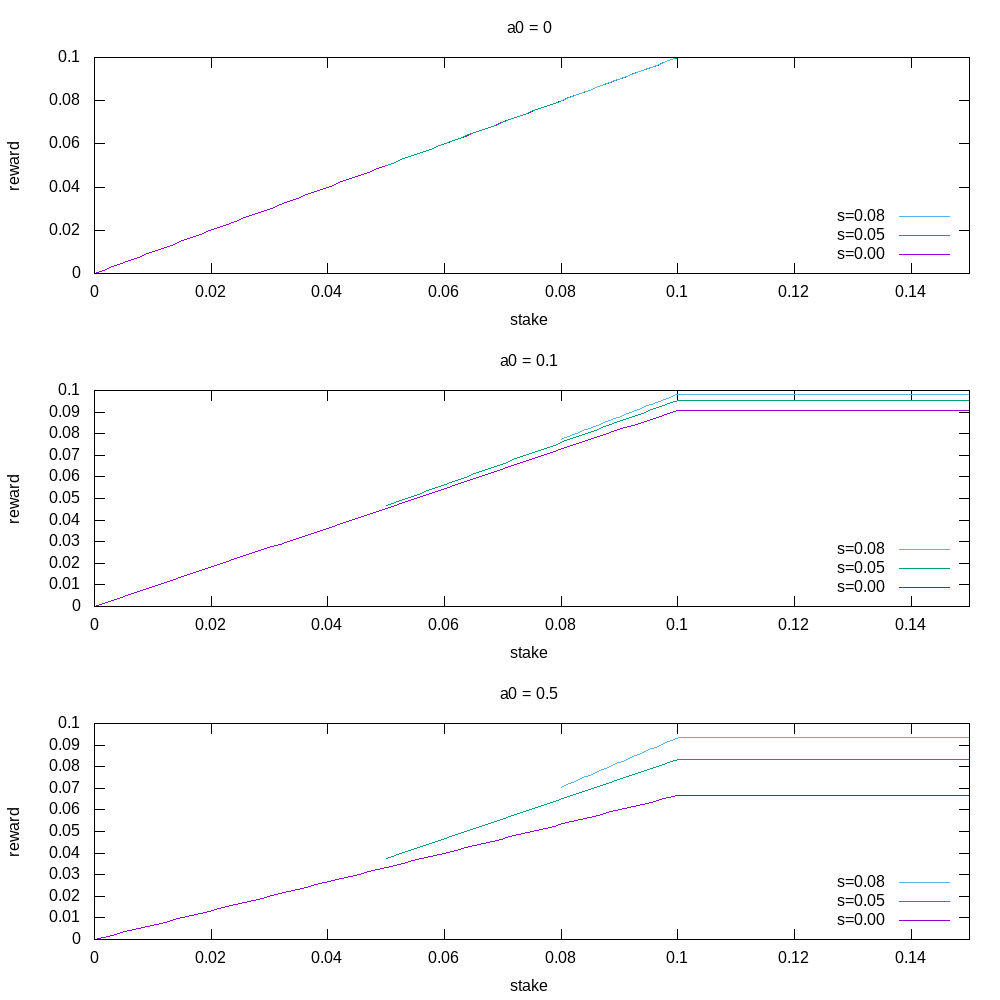
\includegraphics[width=10cm]{rewards.png}
\caption{Effect of different choices for \(a_0\)}
\label{fig:rewards}
\end{figure}

See \cref{fig:rewards} for the effect of various choices for
\(a_0\) on pool rewards (for \(k=10\)).

\subsubsection{\texorpdfstring{\(\rho\)}{\textbackslash{}rho}}

In order to determine the inflation rate per epoch \(\rho\), we need five
more pieces of information:

\begin{itemize}
\item
  The expected \emph{exchange rate} \(e\) from ada to USD (in USD/ADA).
\item
  The average \emph{costs} \(c\) (in USD) to run a pool for one year.
\item
  The average \emph{transaction fees} \(F\) (in ada) paid during one
  epoch.
\item
  The expected ratio \(r\) of \emph{rewards} per year per staked ada.
\item
  The expected value of $\eta$, the ratio of actually produced blocks
  versus expected produced blocks (see~\ref{monetary-expansion}).
\end{itemize}

The available rewards for one epoch (assuming an equilibrium state with
\(k\) pools and noticing that there are \(\frac{365}{5}=73\) epochs per
year) will be \[
    \left(1-\tau\right)\cdot\bigl(F + \min(\eta,1)\cdot\rho\cdot\left(T\infty - T\right)\bigr) - \frac{k\cdot c}{73\cdot e}.
\] On the other hand, \emph{expected} rewards per epoch are \[
    T\cdot\left(\sqrt[73]{1+r}-1\right).
\] Equating the two, we get \[
    \rho=\frac{T\cdot\left(\sqrt[73]{1+r}-1\right)-(1-\tau)\cdot F+\frac{k\cdot c}{73\cdot e}}
    {\left(1-\tau\right)\cdot\min(\eta,1)\cdot\left(T_\infty-T\right)}.
\] For example, using

\begin{itemize}
\item
  \(k=100\),
\item
  \(T=31,000,000,000\,\mathrm{ada}\),
\item
  \(T_\infty=45,000,000,000\,\mathrm{ada}\),
\item
  \(e=0.5\,\mathrm{USD/ada}\),
\item
  \(c=1,000\,\mathrm{USD}\),
\item
  \(F=2,000\,\mathrm{ada}\),
\item
  \(r=0.05\),
\item
  \(\tau=0.2\) and
\item
  \(\eta=0.9\)
\end{itemize}

we would get \[
    \rho=\frac
        {31,000,000,000\cdot\left(\sqrt[73]{1+0.05}-1\right)-0.8\cdot 2000+\frac{100\cdot 1000}{73\cdot 0.5}}
        {0.8\cdot 0.9\cdot\left(45,000,000,000 - 31,000,000,000\right)}
    \approx
    0.0021.
\] This would correspond to reducing the remaining amount of available
ada by \({1.0021}^{73}-1\approx 0.17=17\%\) per year (which sounds
pretty high\ldots).

\subsubsection{\texorpdfstring{\(\tau\)}{\textbackslash{}tau}}

Setting \(\tau\) is a policy decision; we will probably use
\(\tau=0.2\), i.e.~20\% of available epoch rewards will be sent to the
treasury.

\section{Satisfying the Requirements}
\label{satisfying-the-requirements}

In the following, we describe how the requirements listed in
\cref{requirements} are satisfied by the design in this document.

\begin{description}

\item[\cref{proof-of-eligibility} Proof of Eligibility] The leader election
  process takes delegation into account (\cref{slot-leader-schedule}), so the
  leader schedule will contain the key hash of the pool that is expected to sign
  the block. The operational key certificate will be included in the block
  header.

\item[\cref{visibility-of-delegation-on-the-blockchain} Visibility of Delegation
  on the Blockchain] Delegation via delegation certificates is visible on the
  blockchain. Operational key certificates are only used for hot/cold key
  management within a stake pool. Thus, they are not relevant for the rewards
  sharing process.

\item[\cref{restricting-chain-delegation} Restricting Chain
  Delegation] Chain delegation is properly restricted, as described in
  \cref{chain-delegation}.

\item[\cref{cheap-re-delegation} Cheap Re-Delegation] Re-delegation can
  be performed cheaply by issuing a new delegation certificate.

\item[\cref{neutral-addresses} Neutral Addresses] The design includes
  enterprise addresses (\cref{enterprise-address}), which are
  disregarded by the PoS protocol.

\item[\cref{multi-sig-delegation} Multi-Sig Delegation] By allowing script
  credentials not only for payment, but also for stake credentials, and
  implementing a language for expressing multi-sig conditions, we provide a
  mechanism for multi-sig delegation (see \cref{address-structure}).

\item[\cref{sybil-attack-protection-at-stake-pool-level} Sybil Attack
  Protection at Stake Pool Level] Stake pool owners are expected to
  pledge an amount of stake to their pools that has an influence on
  the rewards for their stake pool, and consequently on the
  position of the stake pool in the listing displayed to stakeholders
  (\cref{stake-pool-registration},
  \cref{display-of-stake-pools-in-the-wallet},
  \cref{reminder-stake-pool-registration}).

  Since this pledge cannot be shared between multiple pools, creating
  $n$ viable stake pools will require funds linear in $n$.

\item[\cref{address-nonmalleability} Address Nonmalleability] Protection against
  the malleability attack, by the wallet, is described in
  \cref{address-recognition-1}.

\item[\cref{public-spending-keys-should-not-be-disclosed-prematurely}
  Public Spending Keys Should not be Disclosed Prematurely] The
  introduction of a dedicated staking key (\cref{address-structure})
  avoids the need to use the payment key for delegation purposes.

\item[\cref{mitigate-key-exposure} Mitigate Key Exposure] Stake pool operators
  are required to use operational key certificates for hot/cold key management,
  as described in \cref{operational-key-certificates}.

\item[\cref{handle-inactive-stake-pools} Handle Inactive Stake Pools]
  Stake pools can be retired via a retirement certificate
  (\cref{stake-pool-registration-certificates}. If a stake pool
  ceases to operate without being properly retired, its members will be
  incentivised to re-delegate: their rewards will start to diminish, and their
  wallet will notify them that the pool they have delegated to is not producing
  blocks anymore \cref{display-of-stake-pools-in-the-wallet}.

  In addition to this, \cref{stale-stake} describes an optional mechanism to
  detect and ignore inactive pools that still have stake.

\item[\cref{avoid-hard-transition} Avoid Hard Transition] As described
  in \cref{transition-to-decentralization}, we will have a smooth
  transition from Byron to Shelley, with the core nodes gradually
  transferring the right and obligation to sign blocks to stake pools.

\item[\cref{change-delegation-without-spending-key} Change Delegation
  Without Spending Key] Delegation of cold wallets is described in
  \cref{delegation-of-cold-wallets}, and does not require having the
  spending key of the cold wallet online.

\item[\cref{master-recovery-key} Master Recovery Key] Wallet recovery
  is described in \cref{wallet-recovery-process}, and does not require
  any information in addition to the master key.

\item[\cref{address-recognition} Address Recognition] Wallets will
  recognise addresses belonging to it by looking at the payment key
  hash part of the address, as described in
  \cref{address-recognition-1}.

\item[\cref{wallet-should-be-runnable-on-independent-devices} Wallet
  should be Runnable on Independent Devices] With the caveats listed
  in that requirement, nothing in this document requires wallets
  running on different devices to share state.

\item[\cref{maintain-privacy} Maintain Privacy] Having an efficient
  delegation mechanism -- and in particular a mechanism where
  delegation is rewarded -- requires a slight compromise on the level
  of pseudonymity, since addresses using the same staking key will be
  linkable. However, users can decide to use a number of different
  accounts, with separate staking keys, if they are willing to pay the
  fees for using multiple staking keys. This will give them a level of
  pseudonymity that is not worse than that in the Ethereum network.

  They can also choose to use a distinct staking key per address, or addresses
  with no staking key at all, which gives pseudonymity that is no worse than in
  Bitcoin.

\item[\cref{short-addresses} Short Addresses] The goal of having
  reasonably short addresses has guided the design of delegation, and
  we do not see an obvious way of making them even shorter, while
  still satisfying the rest of the requirements.

\end{description}

\appendix

\section{Assessment of Rewards Sharing Mechanisms}
\label{assessment-of-rewards-sharing-mechanisms}

This appendix gives an overview over the different mechanisms for
rewards sharing that we took into consideration. While this is not
needed for implementing the delegation system, the information is
still useful enough to be included in this document. Choosing a
mechanism for rewards sharing involves a number of non-trivial
trade-offs, and future systems might want to pick one that we
discarded for Cardano.

\subsection{General Considerations}
\label{general-considerations}

\begin{enumerate}
\item
  We use HD Wallets to provide some level of anonymity to stakeholders.
  We would not like to abandon this anonymity for the ability to share
  rewards.

  \begin{itemize}
  \item
    To preserve this level of anonymity HD wallet users will need to
    associate separate staking keys with each HD wallet generated
    address.
  \end{itemize}
\item
  We wish to avoid arbitrary growth in the UTxO (or any other globally
  replicated record, e.g. contents of epoch boundary blocks).

  \begin{itemize}
  \item
    This is potentially at odds with the rewarding of all stakeholders
    at all epochs
  \end{itemize}
\item
  We want to avoid creating dust (entries in the UTxO that are so small
  that including them in a transaction is not economical, since their
  balance is close to or even less than the increase in fees resulting
  from including another input).

  \begin{itemize}
  \item
    The systemic issue is that dust is likely to have an unbounded
    lifetime in the UTxO
  \item
    Transaction fee structure could be modified to remove the
    transaction cost constraint. The requirement on action by the
    receiver still remains.
  \end{itemize}
\item
  The network has a finite capacity to process transactions. We should
  avoid using a significant fraction of this capacity for sharing
  rewards. In particular, we want to avoid causing unreasonable spikes
  in the transaction rate. Those could either bring the system down on
  their own, or act as an invitation to a timed DoS attack.
\item
  The stake pool operator should not be required to take an action to
  initiate sharing rewards with members.
\item
  Verifying that a reward is legitimate will require a node to access
  some information (like the leader schedule of the epoch in which the
  reward was earned, as well as the delegation pattern at the time the
  leader election for that epoch took place). The time and space
  complexity for this should be constant in the size of the blockchain
  and/or the UTxO of non-reward entries.
\end{enumerate}

Unless we want to give up on anonymity (1.), each address has to
separately receive rewards. Together with 2., 3., and 4., this severely
restricts any approach that distributes rewards using ordinary
transactions.

\subsubsection{Hierarchy of desirability of reward distribution}
\label{hierarchy-of-desirability-of-reward-distribution}

\begin{itemize}
\item
  Reward stakeholders on the basis of their holding at an epoch boundary

  \begin{itemize}
  \item
    Stakeholders are not explicitly represented - there can be a proxy
  \item
    One representation of stake delegation (direct to stake pool) which
    has the property of anonymity-via-aggregation. This, combined with
    the desire to not require stake pools to do the distribution a UTxO
    centric reward distribution mechanism.
  \end{itemize}
\item
  Reward stakeholders that ~maintain a UTxO/stake over the total epoch
  length.

  \begin{itemize}
  \item
    This may be seen a ``regressive'' property in that it would not
    reward those stakeholders who engage in high-velocity value
    movements (e.g make use of the HD wallet).
  \item
    This is a property of certain solutions.
  \end{itemize}
\end{itemize}

\subsubsection{Summary of key points of when rewards are calculated}
\label{summary-of-key-points-of-when-rewards-are-calculated}

\begin{itemize}
\item
  Point in Time

  \begin{itemize}
  \item
    Just considers addresses at an epoch boundary
  \end{itemize}
\item
  Duration in Time

  \begin{itemize}
  \item
    Set of stakeholder address and pool arrangement is fixed at an epoch
    boundary (say epoch \(N-1\) to epoch \(N\))
  \item
    Rewards are calculated at the transition from epoch \(N\) to epoch
    \(N+1\)
  \item
    Only stakeholder addresses that have non-zero associated value at
    the epoch \(N\) to \(N+1\) boundary (i.e have ~value at both the
    epoch \(N-1\) to \(N\) and the epoch \(N\) to \(N+1\) boundaries)
    will be eligible to receive rewards

    \begin{itemize}
    \item
      Noting that this could interact badly with HD wallet users
    \end{itemize}
  \end{itemize}
\end{itemize}

\subsection{Approaches that are Ruled Out}
\label{approaches-that-are-ruled-out}

\subsubsection{Manual Sharing}
\label{manual-sharing}

In this approach, only stake pool operators are rewarded directly by the
system, and it is their responsibility to share rewards with members of
the pool.

This approach has been ruled out, since it:

\begin{enumerate}
\item
  requires additional trust in stake pool operators to do this correctly
  (5.)
\item
  requires at least stake pool operators to group the addresses of each
  member, to keep the volume of transactions somewhat reasonable (1.,
  2., 3., and 4.)
\item
  The rewards for members that did not contribute much stake are likely
  to be dust (3.)
\end{enumerate}

\subsubsection{Automatically Issue Transactions Each Epoch}
\label{automatically-issue-transactions-each-epoch}

In this approach, the system automatically distributes rewards at the
end of an epoch, by sending transactions with outputs to every address
that delegated to a stake pool that produced at least one block during
that epoch.

This approach has been ruled out, since it:

\begin{enumerate}
\item
  Leads to a super-linear growth of the UTxO, creating an output per
  address per epoch (2.)
\item
  Is likely to create lots of dust for small stakeholders (3.)
\item
  Will lead to a huge burst of transactions, proportional to the number
  of addresses with non-zero balance in the system (4.). This could be
  lessened somewhat by sending the transactions over the course of the
  following epoch, but it would still use up a large fraction of the
  system's ability to process transactions (4.)
\end{enumerate}

\paragraph{Complexity}

\begin{itemize}
\item
  Creates one ``UTxO'' per non-zero address at the boundary/duration -
  this would create (today) \textasciitilde{}650k transactions per epoch
\end{itemize}

\subsubsection{Let Members Collect Rewards}
\label{let-members-collect-rewards}

An alternative is to let every stake pool member be responsible for
collecting their own rewards. This approach has the virtue that members
could wait several epochs until they had accumulated enough rewards to
warrant a transaction. The overall rate of transactions for sharing
rewards would be reduced, the transactions would not come in bursts, and
the problem of creating dust could be avoided.

However, this approach has been ruled out, since it:

\begin{enumerate}
\item
  Requires nodes to cache or quickly retrieve the whole history of
  leader schedules, as well as the delegation configurations at the time
  of each leader selection (6.)
\end{enumerate}

\subsection{Feasible Approaches}
\label{feasible-approaches}

\subsubsection{Automatic UTxO Updates}
\label{automatic-utxo-updates}

This unique approach circumvents the problems of transaction rates, dust
entries, and UTxO growth, at the expense of introducing an implicit
modification of the UTxO set.

After an epoch, each UTxO entry that delegated to a stake pool will have
its balance updated to reflect the rewards that it earned. Since the
update can be derived from information that every node has (leader
schedule and delegation pattern at the last election), it can be carried
out by each node individually.

Sadly, this approach does come with its own drawbacks:

\begin{enumerate}
\item
  It is not yet clear how a lightweight wallet would determine the
  correct UTxO set.
\item
  It introduces an implicit update of each UTxO entry, a huge moving
  part that makes it much harder to reason about the system.
\item
  Transactions that are formed before an update, but included after it,
  will have a larger total input than the issuer anticipated.
\item
  (Public Perception) This may be perceived as subverting the notion of
  immutability of the blockchain (at least in its UTxO model)
\end{enumerate}

\subsubsection{Lotteries per Stake Pool}
\label{lotteries-per-stake-pool}

A variation of ``Automatically Issue Transactions Each Epoch'', this
approach avoids dust and creating a huge number of transactions by
performing one lottery per stake pool. A number of winning addresses is
determined, and the rewards are distributed amongst those addresses. The
probability of any address winning the lottery is proportional to the
stake that that address contributed to the pool. Benefits of this
approach are:

\begin{enumerate}
\item
  The number of transactions will be proportional to the number of stake
  pools that signed at least one block, which is nicely bounded by the
  number of slots in an epoch.
\item
  The chances of creating dust entries is fairly low, since each winning
  address will receive a sizeable fraction of the pools rewards.
\item
  There is no need to group addresses per stake pool member.
\item
  Possibly -- this would have to be investigated by legal -- this could
  make ada less like a security.
\end{enumerate}

The remaining drawbacks are:

\begin{enumerate}
\item
  It will still create a burst of transactions. This could be prevented
  by staggering the transactions that share rewards
\item
  An individual stake pool member will on average receive the same
  rewards as with any of the other approaches, but it will be much less
  predictable. This might be problematic from a Public Perception
  perspective.
\item
  (Public Perception) although (in the limit) this is the same outcome
  as sharing, apparently most humans don't see things that way\footnote{See
  Prospect Theory (https://en.wikipedia.org/wiki/Prospect\_theory)} --
  they would prefer known outputs (even if smaller) to unknown ones.
  An additional indicator of human response might be to look at a
  similar mechanism (random rewards for depositing a fixed stake) has
  run since 1956. Premium
  Bonds\footnote{https://en.wikipedia.org/wiki/Premium\_Bond} --
  computer nerds /
  crypto nuts should note who helped create the original ERNIE). The
  public might like the gambling aspect, businesses might not!
\end{enumerate}

\subsubsection{Reward accounts per staking key}
\label{reward-accounts-per-stake-key}

This is in some sense a variation of the ``Automatic UTxO updates'', but
trying to address its shortcomings.

Add a new class of address, reward addresses, based on a staking key.
These addresses have special rules:

\begin{itemize}
\item
  Account style accumulation, not UTxO style
\item
  Paid into only by reward payout mechanism, never by normal Txs.
\item
  Withdrawn from by normal Txs, using the staking key as the witness.
\end{itemize}

At the end of an epoch once the pool rewards are known, identify all the
staking keys that contribute to a pool and the rewards per staking key. The
system implicitly issues a transaction/state-change to pay out rewards
to each staking key reward account. These rewards accumulate if they are
not withdrawn.

Value held in a reward account contributes to stake that is delegated to a stake
pool and hence itself attracts rewards. This reduces the incentive to withdraw
early and means the stake corresponding to the reward is not effectively
offline.

Withdrawal of rewards is done similarly to the withdrawal transaction from the
Chimeric Ledgers paper. This uses the staking key as the witness, which reveals
the public part of the staking key. Note that we also require at least one UTxO
input to the transaction for replay protection (see
\cref{certificate-replay-prevention}, \cref{distributing-rewards}).

This aggregation of rewards -- account style -- is the key to resolving
the UTxO storage asymptotic complexity problem. It is the same
fundamental approach as the ``Automatic UTxO updates'' approach, but
putting the aggregation off to into a separate class of addresses, so
that normal addresses remain in a pure UTxO style.

The asymptotic storage complexity of the ledger state (i.e.~UTxO size)
is linear in the number of staking keys, but is unrelated to the number of
epochs that have passed. This is in contrast to approaches that create
UTxO entries for rewards on every epoch.

An important constraint for this approach is that is relies on stake
keys belonging to stakeholders. This means every stakeholder address
must be associated with some staking key belonging to the stakeholder.
This means it is not possible to use addresses that point directly to a
stake pool and still be able to have a corresponding reward address,
since there is not staking key to use for that reward address. There are
alternatives to using addresses that point directly to pools, but these
either reduce privacy or increase fees. One alternative that reduces
privacy is for all addresses in a wallet to share the same staking key
(either as base addresses, or a base address and pointer addresses to
that staking key). This reduces privacy since all addresses in the wallet
can be tied together by using the same staking key. Another alternative is
to use a separate staking key for every address. This means using one
delegation certificate per address. This increases the fees for creating
addresses in a wallet following this policy, and for changing delegation
choices. In principle there's a sliding scale between the two previous
option , using a number of staking keys, more than one but fewer than the
number of addresses.

\begin{itemize}
\item
  stake in reward accounts is ordinary stake, and hence is counted in
  delegation to stake pools.
\item
  There is a potential interaction with UTxO deposit/refund approach. It
  may be that (because the refund is smaller than the reward) that
  negative values need to be stored. Though this may be able to done by
  some registration cost.
\end{itemize}

Advantages:

\begin{itemize}
\item
  doesn't ``mutate'' the UTxO. This reduces conceptual and
  implementation complexity. It does not disrupt wallets and other
  things based on the UTxO model.
\end{itemize}

Disadvantages:

\begin{itemize}
\item
  introduces limited degree of account style chimeric ledgers. This adds
  a degree of conceptual and implementation complexity.
\item
  Cannot use pointer addresses directly to stake pools. Increases fee
  and complexity cost of maintaining wallet privacy.
\item
  Unless people stick to a single staking key (which would immediately
  mean they give up all privacy, not a choice most people would be
  comfortable with I suspect), we basically end up creating lots of
  staking keys, to which we would only deposit once, and withdraw from
  once -- in other words, we'd have reinvented UTxO entries, and the
  accumulation does not help.
\end{itemize}

\section{Deposits}
\label{deposits}

\subsection{Motivation}

One fundamental raison-d'\^{e}tre for transaction fees in Cardano (or any other
cryptocurrency for that matter) is to compensate node operators for their costs:
Processing a transaction incurs costs, and the person doing the processing
should be reimbursed accordingly.

In reality however, there are more than just one-time processing costs.
In particular, there are long term \emph{storage} costs whenever a transaction
forces a node to dedicate local storage for the stake associated with the
transaction.

The prototypical example for this are \emph{UTxO-entries}: Each additional such entry
takes up storage on each node running the protocol.
There are other examples as well, including \emph{stake pool registrations} and
\emph{delegation certificates}.

We plan to address this issue by requiring a \emph{deposit} to be paid for each
resource that will incur storage costs.

This deposit must be (partially) \emph{refundable},
so that the holder of the resource has an incentive to release the resource when
it is no longer needed. So for example, somebody with a lot of ``dust'' in their
wallet would have an incentive to remove that dust, thus reclaiming some of the
deposit paid for UTxO-entries.

On the other hand, refunds should also \emph{decrease over time}, so that
there is an incentive to release a resource sooner rather than later.

\subsection{Mechanism}

We propose to introduce the following configurable parameters:
\begin{enumerate}
    \item
        A deposit amount (in ada) $d_R\in(0,\infty)$ for each type of resource
        $R$. The value of $d_R$ for a resource type $R$ should roughly reflect
        the cost to ``rent the resource forever''.
    \item
        A factor $d_{\min}\in(0,1)$, which determines the minimal proportion of
        $d_R$ that will be refunded on resource release. Higher value of
        $d_{\min}$ mean higher guaranteed refunds.
    \item
        A decay constant $\lambda\in(0,\infty)$ determining how refunds decrease
        over time. Higher values of $\lambda$ correspond to faster decrease of
        refunds over time.
\end{enumerate}

Given these parameters, on acquiring a resource of type $R$, one would have to
pay an amount of $d_R$ ada\@. When the resource is released after $t\geq 1$ slots,
the holder of the resource is refunded
\[
    r_R(t)=d_R\cdot\left(d_{\min}+(1-d_{\min})\cdot e^{-\lambda t}\right)\in(d_{\min}\cdot d_R,d_R),
\]
whereas the difference $d_R-r_R(t)$ is added incrementally to the reward pools of
the epochs between registering and releasing the resource.

Note that it easily follows from well-known properties of the exponential
function that
\[
    d_r>r_R(t)\stackrel{t\rightarrow\infty}{\xrightarrow{\hspace{10mm}}}d_{\min}\cdot d_R,
\]
as desired.

As a fictional example, consider parameter values $d_{\min}=0.25$ and $\lambda=0.0001$
and a resource of type $R$ with $d_R=2$. A user acquiring such a resource
will initially include a deposit of $d_R=2$ ada in the transaction creating that
resource. This deposit will be held in escrow until the resource gets released.
If the user releases the resource after 10,000 slots, a refund of
$r_R(10,000)=1.0518$ ada will be added to the available input of the associated
transaction. The difference $d_R-r_R(10,000)=2-1.0518=0.9482$ ada will be added
to the rewards pool of that epoch.

If our fictional user held onto the resource for 40,000 slots instead,
their refund would only be $r_R(40,000)=0.5275$ ada, and 1.4725 ada
would be added to the epoch rewards. In this example, refunds will
never drop below $d_{\min}\cdot d_R=0.5$ ada.

\section{Design Option: Stale Stake}
\label{stale-stake}

This section sketches an optional mechanism for tracking \emph{stale
  stake}, i.e., stake that is no longer being actively
controlled. Stale stake can limit the chain growth (since elected
leaders might fail to show up and sign blocks), and decrease the
amount of honest stake, making the system easier to attack. The
mechanism described below is aimed at mitigating the first effect.

In the current design, stale stake is much less likely to become a
problem than in earlier iterations (since we automatically discard
stake that is not delegated to a valid stake pool), so we propose to
not implement this design option, at least not in the initial Shelley
release. We keep it in this document for further reference.

In the current design, the only circumstance where an actor becoming inactive
would limit the chain growth is when a stake pool operator ceases to operate
their pool, without retiring it. Furthermore, since a failure to produce blocks
will reduce the rewards for stake pool members, such a pool would lose members
and become irrelevant. Thus, an abandoned pool will be an impediment to chain
growth only if there are stakeholders delegating to that pool who also become
inactive and do not re-delegate.

In order to further mitigate this potential problem, the system could monitor
the apparent performance of all pools over time, and prune pools that fulfill
both of the following conditions:

\begin{itemize}
  \item The apparent performance of the pool has consistently been zero for a
    certain number of epochs (i.e., the block did not produce any blocks after a
    certain moment in time).
  \item The pool has enough stake that it should have been elected as slot
    leader within those epochs several times.
\end{itemize}

The number of epochs and size in stake should be such that we can rule out the
hypothesis that the pool is still active, but was just not elected as leader
during those epochs, with statistical significance\footnote{Setting those
  numbers would require some research if we were to implement this feature.}.

We do not anticipate that abandoned pools should become a problem anytime soon.
By monitoring the chain growth, we could detect whenever a significant fraction
of pools accumulates in abandoned pools, and implement abandoned pool detection
when necessary.

\section{FAQ}

\subsection{Why will stake pools accept new stake pool registration
  certificates?}

It may seem counterintuitive that any of the existing stake pools would accept a
stake pool registration certificate for a new pool, for fear of losing some of
their future rewards to the increased competition. After all, with a naive
approach to rewarding pools, a new pool would potentially reduce the rewards of
every existing pool. Existing systems like Bitcoin tend to becoming more
centralised because they use naive incentives.

One thing to realise is that Cardano uses a sophisticated incentives scheme
\citep{bkks2018}, summarised in \cref{design-of-incentives}, where the system
tends to a fixed number \(k\) of saturated stake pools, and no pool can increase
their own rewards by trying to reduce the number of active pools below \(k\). So
there is no general incentive, that would cause every stake pool to try to
censor the registration of a new pool.

The operator of a pool that is near the bottom of the list of competitive pools
might fear to be replaced by a new pool, and it would not be unreasonable for
that operator to try to prevent new pools from registering. But since it only
takes a \emph{single pool} to include the certificate\footnote{%
  To be precise, this also requires that a majority of players is going to
  accept a block that contains a certificate. But dropping a block because it
  contains a certificate is much worse than just not including the certificate
  in a block: it creates a fork and thereby attacks the integrity of the system,
  and a pool doing that risks losing their own block when the fork is resolved.
  Also, a pool that repeatedly creates a fork after a block that contains a
  stake pool registration certificate would sooner or later be detected and
  blamed by the community},%
there is no hope to achieve this, and the rational behaviour is to just play by
the rules and include the certificate.

The situation where each pool accepts submitted certificates is a \emph{Nash
  Equilibrium}, where no player can benefit from deviating from this behaviour.
Such configurations are stable, since getting to a different state requires
either collusion between a large number of players, or players acting
irrationally against their own interests.

However, there is a subtlety here: the state where \emph{no} pool accepts new
certificates might also be a Nash Equilibrium: in this case, pools may refrain
from entering a new certificate for fear to lose rewards due to increased
competition, which will either kick them out of the \(k\) best pools or lower
their margins.

Let us call the former equilibrium, where certificates are accepted, NE1, and
the latter, where they are rejected, NE2. Should we be worried that the system
will end up in NE2? There are three arguments why this is unlikely to happen:

\begin{itemize}
\item When the system is initially decentralised, a majority of blocks will be
  created by the federation that ran the Byron network, and those players will
  behave honestly. So the system will start in NE1.
\item Stake pool \emph{members} benefit from competition, and while censorship
  of certificates is not observable from the final chain itself, the community
  can be expected to identify pools that try to block the competition, by
  looking at the certificates that are being broadcast, the produced blocks, and
  temporary forks. Once this becomes known, members will leave such a pool. So
  there is a high risk involved for stake pools.
\item Last but not least, the project is run by a community, and it is not
  unreasonable to expect members to be at least somewhat cooperative.
\end{itemize}

\subsection{Won't stake pools reject delegation certificates that delegate away
  from them?}

That would only work if a majority of stake pools colluded to censor such a
certificate. But all pools are incentivised to include the certificate, via
fees. So this censorship would only happen if a majority of pools decided to
partake in malicious behaviour and attack the system, against their direct
incentives.

\section{Transaction Metadata}

Adding metadata to transactions is a useful new feature in Cardano Shelley.
It is not related to delegation or decentralisation.

\subsection{Motivation and design goals}

The purpose is to enable a range of new applications by allowing arbitrary
structured data to be included onto the chain, and to make effective use of
that data. The term `metadata' is perhaps a misnomer since it is simply about
placing application specific data on the chain; it is only metadata from the
point of view of a transaction since it is carried along with transactions and
not involved in validation.

A design goal is to add very little complexity to the on-chain part of the
system but to get (or allow for) as much functionality as possible, in
combination with other features or components. This helps keep implementation
complexity lower. Importantly it keeps the size of the trusted base low, by
having the complex functionality to use the metadata outside of the trusted
base.

A design principle that we preserve is that the historical data on the chain is
not needed to validate the next block or transaction. All data needed for later
validation must be explicitly tracked in the ledger state. This means the old
part of the chain does not need to be preserved locally at all, or at least not
in random access storage. This avoids a problem that Ethereum ran into with
disk I/O becoming a performance bottleneck. This is why the design does not
include metadata into the ledger state, and does not make it accessible to
later scripts.

\subsection{Detail}

The transaction can contain metadata. The metadata hash is part of the body of
the transaction so is covered by all transaction signatures. This allows for
integrity checking and authentication of the metadata.

The metadata value is kept outside of the transaction body, much like the
transaction witnesses. This follows the `segmented witness' design idea that
allows witnesses to be discarded when the data is known to have been checked.
We go one step further and keep the metadata outside the body separately from
the witnesses too, in principle allowing an implementation to store or discard
the metadata or the witnesses independently of each other.

The structure of the metadata is a mapping from keys to values. The keys are
unsigned integers limited in size up to 64 bits. The values are simple
structured terms, consisting of integers, text strings, byte strings, lists and
maps.

There is no limit on the number of key-value pairs, except that imposed by the
overall transaction size limit. There is also no limit on individual structured
values, but there is a limit on the size of text strings and byte strings
within the structured values.

A key aspect of the design is that metadata included in transactions is not
available for later retrieval from within the ledger validation rules,
including scripts. The metadata is not entered into the ledger state, and
general historical chain data is not otherwise available to the ledger
validation rules.

The changes to the ledger validation rules are thus very limited: only the
metadata syntax, metadata size limits and the effect of the metadata on the
transaction size calculation and thus the transaction fees. No data is added
to the ledger state. The metadata resides only on the chain.

There are no special fees for metadata. The metadata simply contributes to the
size of the transaction and fees are based on the transaction size. This choice
is justified by the fact that the cost to operators is only the one-time
processing cost and any long term storage of the blockchain. There is no long
term random access state.

The metadata within a transaction will be made available to validation scripts,
including Plutus Core scripts. Note again that this is only the immediate
transaction being validated. No metadata from predecessor transactions is
available.

\subsection{Explanation and use}

The purpose of the metadata being a key value mapping is to make it
straightforward to combine metadata for multiple purposes into the same
transaction. Think of the metadata key as being a schema identifier, that
says what the metadata value is. There is however no on-chain schema
enforcement. The interpretation of the data is entirely up to the applications
that consume it.

It may make sense to establish a public registry of known metadata keys and
corresponding schemas.

The metadata value is required to be structured data rather than a single
unstructured blob. The available structure is like a simplified version of JSON.
This makes the data easier to inspect and manipulate, particularly by scripts,
such as Plutus scripts, in future evolutions of the system. The metadata values
do not include floating point numbers because on-chain script languages cannot
support such types.

The size of strings in the structured value is limited to mitigate the problem
of unpleasant or illegal content being posted to the blockchain. It does not
prevent this problem entirely, but it means that it is not as simple as posting
large binary blobs.

Of course posting data to the chain is only half the story. It must also be
possible to use it effectively. Part of the design is that the data is not
kept in random-access storage for use by on-chain scripts, so that validating
the chain does not require random access to old parts of the chain or large
databases. So the design calls for metadata use to be managed off-chain using
an indexing service.

An indexing service, much like an explorer, enables the collection,
authentication and query of the metadata that is posted on the chain. It is
clear that an agent can follow the chain and write all transaction metadata
into a relational database for later query. This is the design that the
backends for many blockchain explorers use. This solves the collection and
query parts of the problem, but not the authentication part.

Using HD wallet schemes however, the authenticity of the metadata can be
ensured. Depending on the HD scheme -- using public or non-public key
derivation -- the metadata can be publicly verifiable, or only privately
verifiable.

For example, a simple scheme to track the issuance of physical items could
involve the original owner posting metadata within transactions that spend from
a designated wallet. An indexing server that knows the HD wallet structure (and
either public or private keys depending on the HD scheme) can track the wallet
and index all the metadata in transactions from that wallet (or wallet
sub-account).

Such schemes have a great deal of flexibility since there is a lot of
flexibility in HD wallet schemes. With public HD derivation, the indexing
server does not need any signing keys, just an appropriate verification key of
a sub-tree in the HD wallet space. If that verification key is revealed then
anyone can reliably run the indexing service, and anyone can verify that the
metadata is authentic. If the verification key is not revealed then only the
owner can run the indexing service, and be used to implement some lookup or
verification service, or it can reveal the authenticity of a particular address
without revealing all addresses.

It is even possible in principle to use multi-signature wallets, or wallets
involving scripts. There just needs to be some wallet scheme that the indexing
service can use to reliably track and authenticate the transactions using the
wallet.

Obviously, to take advantage of these possibilities requires suitable wallet
and indexing components. These are however independent components and their
complexity does not impact the complexity of the on-chain rules, so does not
add to the size of the trusted base of the overall system.

\subsection{Binary schema}

The binary schema is very simple. The notation is CBOR CDDL (much like BNF).

\begin{verbatim}
metadata = { * metadata_key => metadata_value }

metadata_key = uint

metadata_value =
    int
  / bytes .size 64
  / text  .size 64
  / [ * metadata_value ]
  / { * metadata_value => metadata_value }
\end{verbatim}

\addcontentsline{toc}{section}{References}
%\bibliographystyle{plainnat}
\bibliographystyle{habbrv}
\bibliography{references}

\end{document}

%%% Local Variables:
%%% mode: latex
%%% TeX-master: t
%%% End:
